%\title{Rapport_stage_M2}
%----------------------------------------------------------------------------------------
%	PACKAGES AND OTHER DOCUMENT CONFIGURATIONS
%----------------------------------------------------------------------------------------

\documentclass[12pt]{report}
\usepackage[english]{babel}
\usepackage[utf8x]{inputenc}
\usepackage[fleqn]{amsmath}
\usepackage{amssymb}
\usepackage{graphicx}
\usepackage[colorinlistoftodos]{todonotes}
\usepackage{geometry}
\geometry{hmargin=2.0cm,vmargin=1.5cm}
\usepackage{wrapfig}	% Figures avec du texte autour
\usepackage{lipsum}
\usepackage{array}

%%%% debut macro %%%%
\newenvironment{changemargin}[2]{\begin{list}{}{%
\setlength{\topsep}{0pt}%
\setlength{\leftmargin}{0pt}%
\setlength{\rightmargin}{0pt}%
\setlength{\listparindent}{\parindent}%
\setlength{\itemindent}{\parindent}%
\setlength{\parsep}{0pt plus 1pt}%
\addtolength{\leftmargin}{#1}%
\addtolength{\rightmargin}{#2}%
}\item }{\end{list}}
%%%% fin macro %%%%

\begin{document}

\begin{titlepage}

\newcommand{\HRule}{\rule{\linewidth}{0.5mm}} % Defines a new command for the horizontal lines, change thickness here

\center % Center everything on the page
 
%----------------------------------------------------------------------------------------
%	HEADING SECTIONS
%----------------------------------------------------------------------------------------
\textsc{\LARGE Le Mans Université}\\[1.5cm] % Name of your university/college
\textsc{\Large Rapport de Stage en Laboratoire}\\[0.5cm] % Major heading such as course name
\textsc{\large Master acoustique : Métiers de la recherche en acoustique}\\[0.5cm] % Minor heading such as course title

%----------------------------------------------------------------------------------------
%	TITLE SECTION
%----------------------------------------------------------------------------------------

\HRule \\[0.4cm]
{ \huge \bfseries Caractérisation et conception d'un milieu poreux anisotrope}\\[0.4cm] % Title of your document
\HRule \\[1cm]
 
%----------------------------------------------------------------------------------------
%	AUTHOR SECTION
%----------------------------------------------------------------------------------------

\begin{minipage}{0.4\textwidth}
\begin{flushleft} \Large
\emph{Author:}\\
Arthur \textsc{Terroir} % Your name
\end{flushleft}
\end{minipage}
~
\begin{minipage}{0.1\textwidth}
\end{minipage}
\begin{minipage}{0.5\textwidth}
\Large{\emph{Supervisor:} \\ Pr. Jean-Philippe \textsc{Groby}},\\
\large Chargé de Recherche CNRS.
\end{minipage}\\[1cm]

% If you don't want a supervisor, uncomment the two lines below and remove the section above
%\Large \emph{Author:}\\
%John \textsc{Smith}\\[3cm] % Your name

%----------------------------------------------------------------------------------------
%	DATE SECTION
%----------------------------------------------------------------------------------------

{\large \today}\\[1cm] % Date, change the \today to a set date if you want to be precise

%----------------------------------------------------------------------------------------
%	LOGO SECTION
%----------------------------------------------------------------------------------------
\hspace{2cm}
\begin{minipage}[c]{0.4\linewidth}
\centering
\hspace{-3cm}
\vspace{1.2cm}

\includegraphics[scale=0.9]{logo_LAUM.png}\\[1cm]  
\end{minipage}
\begin{minipage}[c]{0.4\linewidth}
\centering
\hspace{-1cm}
\vspace{1.2cm}

\includegraphics[scale=1.6]{logo_cnrs.jpg}\\[1cm]  
\end{minipage}
\begin{minipage}[l]{0.8\linewidth}
\centering
\hspace{1.3cm}
\vspace{0.5cm}

\includegraphics[scale=0.5]{Logo_LeMansUniv.png}\\[1cm]  
\end{minipage}
\end{titlepage}
%----------------------------------------------------------------------------------------
\begin{abstract}

\end{abstract}
\tableofcontents
\listoffigures

\newpage
\chapter*{Introduction}
\addcontentsline{toc}{chapter}{Introduction} 
\pagenumbering{arabic} \setcounter{page}{1}
   
%%%%%%%%%%%%%%%%%%%%%%%%%%%%%%%%%%%%%%%%%%%%%%%%%%%%%%%%%%%%%%%%%%%%%%%%%%%%%%%%%%%%%%%%%%%%%%%%%%%%%%%%%%%%% 
\chapter{Propagation dans une couche de fluide équivalent anisotrope}
\label{Ch_Prop}
\section{Problème de propagation dans le milieu fluide équivalent}
\label{Ch_Prop_S_Pb}
\subsection{Problème étudié}
\label{Ch_Prop_S_Pb_SS_Pb}
    Le problème étudié dans cette méthode est un problème de propagation dans un milieu fluide équivalent anisotrope, de dimension infinie dans le plan $x_1x_2$ et L selon $x_3$.  La situation est présentée sur la figure \ref{Schema}:
    \begin{figure}[ht!]
    \centering
    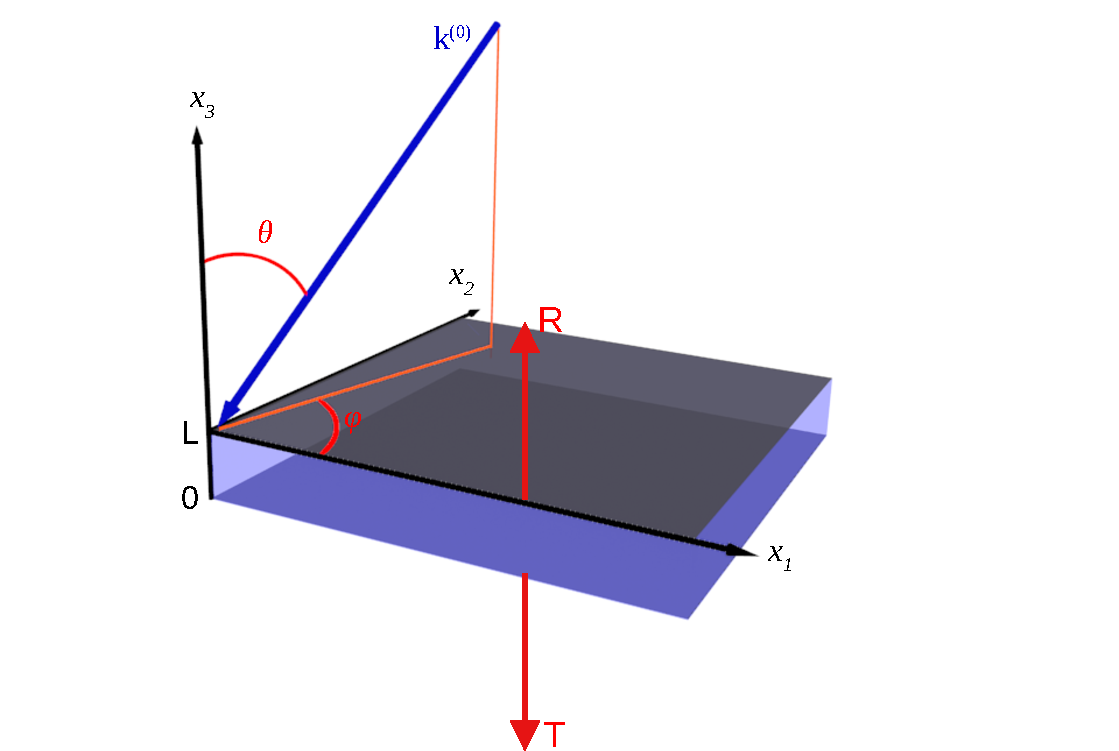
\includegraphics[scale=1]{Fig3D.pdf}
    \caption{Réflexion et transmission dans un milieu fluide équivalent anisotrope. Le milieux est supposé infini dans le plan $x_1x_2$ et de dimension L selon $x_3$. Le fluide est excité avec une onde plane harmonique à l'interface $x_3=L$ et l'on observe une onde transmise en $x_3=0$. }
    \label{Schema}
    \end{figure}
    
    Dans ce problème on s'intéresse aux ondes réfléchies et transmises, soit au coefficient de réflexion et transmission R et T, pour une propagation le long de la direction $x_3$.
    Le fluide est considéré comme anisotrope et, dans le cas de notre étude, hors de ses directions principales. Le milieux étant un fluide équivalent, quelques observations sont à faire, dans un premier temps les grandeurs observées (bulk modulus, denisté) sont considérées comme complexes, dû à la considération de perte. Dans un second temps, ces mêmes grandeurs sont dépendantes de la fréquence.
    Il est donc possible de décrire la couche fluide avec une matrice de densité complexe telle que :
    \begin{align}
    \bar{\bar{\rho}}=\begin{pmatrix}
    					\rho_{11} & \rho_{12} & \rho_{13} \\
                        \rho_{12} & \rho_{22} & \rho_{23} \\
                        \rho_{13} & \rho_{23} & \rho_{33}                       
    				 \end{pmatrix}.
    \end{align}
    et d'un bulk modulus $K$.
    
    Le milieu est excité par une onde plane harmonique, d'amplitude 1, de pulsation $\omega$, d'angle d'incidence d'élévation $\theta$ et azimutal $\phi$. Les projections du nombre d'onde $k^{(0)}$ peuvent donc s'exprimer comme : 
    \begin{align}
    &k_1=-k_0 sin(\theta) cos(\phi),\label{k1} \\
    &k_2=-k_0 sin(\theta) sin(\phi),\label{k2} \\
    &k_3= -k_0 cos(\theta),\label{k3}
    \end{align}
        
        Le problème étant posé on s'intéresse maintenant au problème de propagation.
        
\subsection{Propagation dans le milieu fluide équivalent anisotrope}
\label{Ch_Prop_S_Pb_SS_Eul}
    Les équations constitutives suivantes sont considérées :
    \begin{align}
	&\rho \frac{\partial}{\partial t}v=-\nabla p,\label{Const1} \\
	&\frac{\partial}{\partial t}p=-K\nabla v.\label{Const2}
    \end{align}
    Les solutions à ces équations dans la couche fluide sont supposées être  des ondes planes harmoniques telles que, en posant la convention temporelle $e^{i\omega t}$, l'on puisse écrire dans le domaine $0<x_3<L$ :
    \begin{align}
        \xi=\tilde{\xi}e^{i(k_1 x_1+k_2 x_2)}e^{-i\omega t}\label{Convention_k_t}
    \end{align}
    Le vecteur d'état $\bar{S}$ est ici introduit tel que $\bar{S}=\begin{pmatrix} p \\ v_3 \end{pmatrix}$, $\bar{S}$ permet de caractériser la propagation le long de la direction $x_3$, et ainsi d'obtenir la matrice de transfère $Tr$ du fluide entre les deux interfaces.
    
    En introduisant un champs de pression de la forme (\ref{Convention_k_t}) dans les équations (\ref{Const1}) et (\ref{Const2}), il vient :
    \begin{align}
	&ik_ip=\sum_{j=1}^{3} i \omega \rho_{ij} v_j,\ i=1,2\label{Euler1}\\
	&\frac{\partial}{\partial x_3}p=\sum_{j=1}^{3} i \omega \rho_{3j} v_j\label{Euler2}\\
    &i\omega p= iK(k_1v_1+k_2v_2+\frac{\partial}{\partial x_3}v_3).\label{Euler3}
    \end{align}
	En utilisant l'expression (\ref{Euler1}), il est possible d'écrire $v_1$ et $v_2$ en fonction de $p$ et $v_3$, comme :
    \begin{align}
	v_1=\frac{1}{\rho_{11}-\frac{\rho_{12}^2}{\rho_{22}}}([\frac{k_1}{\omega}-\frac{\rho_{12}}{\rho_{22}}\frac{k_2}{\omega}]p+[\frac{\rho_{12}}{\rho_{22}}\rho_{23}-\rho_{13}]v_3), \\
	v_2=\frac{1}{\rho_{22}-\frac{\rho_{12}^2}{\rho_{11}}}([\frac{k_2}{\omega}-\frac{\rho_{12}}{\rho_{11}}\frac{k_1}{\omega}]p+[\frac{\rho_{12}}{\rho_{11}}\rho_{13}-\rho_{23}]v_3).
    \end{align}
 	Ce qui permet d'exprimer $\frac{\partial}{\partial x_3}v_3$ et $\frac{\partial}{\partial x_3}p$ comme $\frac{\partial}{\partial x_3}v_3(p,v_3)$ et $\frac{\partial}{\partial x_3}p(p,v_3)$, en introduisant ces expressions dans les équations (\ref{Euler2}) et (\ref{Euler3}), il est donc possible d'écrire :
    \begin{align*}
    \frac{\partial}{\partial x_3}v_3=&[\frac{i\omega}{K}-\frac{ik_1}{\rho_{11}-\frac{\rho_{12}^2}{\rho_{22}}}(\frac{k_1}{\omega}-\frac{\rho_{12}}{\rho_{22}}\frac{k_2}{\omega})-\frac{ik_2}{\rho_{22}-\frac{\rho_{12}^2}{\rho_{11}}}(\frac{k_2}{\omega}-\frac{\rho_{12}}{\rho_{11}}\frac{k_1}{\omega})]p\\
    &-[\frac{ik_1}{\rho_{11}-\frac{\rho_{12}^2}{\rho_{22}}}(\frac{\rho_{12}}{\rho_{22}}\rho_{23}-\rho_{13})+\frac{ik_2}{\rho_{22}-\frac{\rho_{12}^2}{\rho_{11}}}(\frac{\rho_{12}}{\rho_{11}}\rho_{13}-\rho_{23})]v_3,
    \end{align*}
    et 
    \begin{align*}
    \frac{\partial}{\partial x_3}p=&[\frac{i\omega \rho_{13}}{\rho_{11}-\frac{\rho_{12}^2}{\rho_{22}}}(\frac{k_1}{\omega}-\frac{\rho_{12}}{\rho_{22}}\frac{k_2}{\omega})+\frac{i\omega \rho_{23}}{\rho_{22}-\frac{\rho_{12}^2}{\rho_{11}}}(\frac{k_2}{\omega}-\frac{\rho_{12}}{\rho_{11}}\frac{k_1}{\omega})]p\\
    &+[\frac{i\omega \rho_{13}}{\rho_{11}-\frac{\rho_{12}^2}{\rho_{22}}}(\frac{\rho_{12}}{\rho_{22}}\rho_{23}-\rho_{13})+\frac{i\omega \rho_{23}}{\rho_{22}-\frac{\rho_{12}^2}{\rho_{11}}}(\frac{\rho_{12}}{\rho_{11}}\rho_{13}-\rho_{23})]v_3.
    \end{align*}
    
    Sous forme matricielle, il est possible d'exprimer la matrice de propagation $\bar{\bar{A}}$ permettant de décrire l'évolution du vecteur d'état $\bar{S}$. Le problème de propagation prend donc la forme suivante :
    \begin{align}
    \frac{\partial}{\partial x_3}\bar{S} = \bar{\bar{A}} \bar{S},\label{Equa_diff}
    \end{align}
    avec $\bar{\bar{A}}$ la matrice de propagation telle que :
     \begin{align}
     &\bar{\bar{A}}=\begin{pmatrix}
    				A_{11} & A_{12} \\ A_{21} & A{22}
    			\end{pmatrix}\label{Matrice_complete},\\ 
     &A_{11}=A_{22}=i[\frac{\rho_2\rho_{13}-\rho_{12}\rho_{23}}{\rho_1\rho_2-\rho_{12}^2}k_1+\frac{\rho_1\rho_{23}-\rho_{12}\rho_{13}}{\rho_1\rho_2-\rho_{12}^2}k_2], \\
     &A_{12}=i\omega \rho_3[1-\frac{\rho_{13}}{\rho_1\rho_2-\rho_{12}^2}(\frac{k_1^{(i)}}{k_3^{(i)}})^2(\rho_2-\rho_{12}(\frac{k_2^{(i)}}{k_1^{(i)}})^2)-\frac{\rho_{23}}{\rho_1\rho_2-\rho_{12}^2}(\frac{k_2^{(i)}}{k_3^{(i)}})^2(\rho_1-\rho_{12}(\frac{k_1^{(i)}}{k_2^{(i)}})^2)], \\
     &A_{21}=\frac{i\omega}{K}[1-\frac{\rho_3}{\rho_1\rho_2-\rho_{12}^2}(\frac{k_1}{k_3^{(i)}})^2(\rho_2-\rho_{12}\frac{k_2}{k_1})-\frac{\rho_3}{\rho_1\rho_2-\rho_{12}^2}(\frac{k_2}{k_3^{(i)}})^2(\rho_1-\rho_{12}\frac{k_1}{k_2})],
    \end{align}
    ou $k_m^{(i)},\ i=1,2,3$ sont des nombres d'onde effectifs selon la direction $x_i$, ne dépendant pas de la fréquence et de l'angle d'incidence.
    
	L'expression (\ref{Matrice_complete}) permet de décrire quatre paramètres liés à la propagation dans la couche fluide équivalente anisotrope, un Bulk modulus équivalent effectif $\tilde{K}$ lié à la direction de propagation et au Bulk modulus équivalent, une densité effective $\tilde{\rho_3}$ liée à la propagation des ondes selon $x_3$, et deux termes de phase $q_1$ et $q_2$, respectivement liés à $k_1$ et $k_2$, issus du couplage induit par les termes extra-diagonaux. Ces paramètres sont décrits ci-dessous :
    \begin{align}
     &\tilde{K}=\frac{K}{[1-\frac{\rho_{33}}{\rho_{11}\rho_{22}-\rho_{12}^2}(\frac{k_1}{k_3^{(i)}})^2(\rho_{22}-\rho_{12}\frac{k_2}{k_1})-\frac{\rho_{33}}{\rho_{11}\rho_{22}-\rho_{12}^2}(\frac{k_2}{k_3^{(i)}})^2(\rho_{11}-\rho_{12}\frac{k_1}{k_2})]}\label{Ktild},\\
     &\tilde{\rho_3}=\rho_{33}[1-\frac{\rho_{13}}{\rho_{11}\rho_{22}-\rho_{12}^2}(\frac{k_1^{(i)}}{k_3^{(i)}})^2(\rho_{22}-\rho_{12}(\frac{k_2^{(i)}}{k_1^{(i)}})^2)-\frac{\rho_{23}}{\rho_{11}\rho_{22}-\rho_{12}^2}(\frac{k_2^{(i)}}{k_3^{(i)}})^2(\rho_{11}-\rho_{12}(\frac{k_1^{(i)}}{k_2^{(i)}})^2)]\label{rho3tild}, \\
	&q_{1}=\frac{\rho_{22}\rho_{13}-\rho_{12}\rho_{23}}{\rho_{11}\rho_{22}-\rho_{12}^2}k_1\label{q1},\\
    &q_{2}= \frac{\rho_{11}\rho_{23}-\rho_{12}\rho_{13}}{\rho_{11}\rho_{22}-\rho_{12}^2}k_2\label{q2}.
          \end{align}
    Quelques commentaires peuvent être formulés à propos des ces paramètres, un premier point est que conformément à des paramètres effectifs, dans un cas isotrope, on retrouve  $\tilde{K}=K$ et $\tilde{\rho_3}=\rho_3$. Il est possible de remarquer, que quelque soit l'anisotropie, en incidence normale, $\tilde{K}=K$. Une autre remarque importante est de voir que $\tilde{\rho_3}$ est indépendant de l'angle d'incidence de l'excitation, contrairement à $\tilde{K}$. Les termes de phase $q_1$ et $q_2$ semblent traduire la variation de phase lors de la transmission de phase due au couplage induit par les densités extra-diagonales, et notamment $\rho_{13}$ et $\rho_{23}$  qu'on pourrait voir comme une rotation du plan principale $x_Ix_{II}$.
    
    Finalement, l'équation différentielle (\ref{Equa_diff}) amène à l'expression suivante : 
    \begin{align}
    \bar{S}_{(L)}=e^{\bar{\bar{A}}L}\bar{S}_{(0)}.\label{PB}
    \end{align}
    La matrice de transfère $Tr$ peut donc être déduite comme $Tr=e^{\bar{\bar{A}}L}$. Si l'expression analytique de la matrice de transfère est connue, c'est-a-dire que l'on puisse diagonaliser la matrice de propagation $\bar{\bar{A}}$, il est alors possible en posant des conditions aux frontières de résoudre le problème réflexion/transmission dans le milieu fluide.
    
    Le calcul de la matrice de transfère du système passe donc par la diagonalisation de $\bar{\bar{A}}$, qui s'écrit :
    \begin{align}
    \bar{\bar{A}}=\bar{\bar{U}} \begin{pmatrix}
    								-ik_{33}+i\tilde{q} & 0 \\ 0 & ik_{33}+i\tilde{q} 
    							\end{pmatrix} \bar{\bar{U^{-1}}}.
    \end{align}
    avec $\tilde{q}=q_1+q_2$ le terme de phase global du système, $k_{33}=\frac{\omega}{c_{33}}$ le nombre d'onde effectif selon $x_3$, $c_{33}=\sqrt{\frac{\tilde{K}}{\tilde{\rho_3}}}$ la célérité dans la direction $x_3$.
    Les vecteurs propres s'écrivent :
    \begin{align}
    &\bar{\bar{U}}=\frac{1}{\sqrt{2}}\begin{pmatrix}
    					Z_3 & Z_3 \\ -1 & 1
    								\end{pmatrix},\\
    &\bar{\bar{U^{-1}}}=\frac{1}{Z_3 \sqrt{2}}\begin{pmatrix}
    					1 & -Z_3 \\ 1 & Z_3
    		   						\end{pmatrix},           
    \end{align}
    avec $Z_3=\tilde{\rho_3}c_{33}$ l'impédance effective du milieu fluide.
    La matrice de transfère $Tr$ peut donc s'écrire :
        \begin{align}
    Tr=\bar{\bar{U}}\begin{pmatrix}
    e^{-ik_{33}L} & 0 \\ 0 & e^{-ik_{33}L} 
    \end{pmatrix} e^{i\tilde{q}L}\bar{\bar{U^{-1}}}\label{Matrice_Transfere}
    \end{align}

\subsection{Conditions aux limites}
\label{Ch_Prop_S_Pb_SS_BC}
    L'onde incidente excitant la couche de fluide équivalent a l'interface $x_3=L$ est supposé de la forme :
    \begin{align}
    p_{(L)}=p\big{|}_{x=L}=1*e^{-i k_3(x_3-L)}+R e^{i k_3(x_3-L)}.
    \end{align}
    De même l'onde transmise à l'interface $x_3=0$ est de la forme : 
    \begin{align}
    p_{(0)}=p\big{|}_{x=0}=Te^{-ik_3x}.
    \end{align}

    La matrice de transfert du milieu étant connue, il faut donc maintenant poser des conditions frontières, dans notre problème on s'intéresse aux ondes réfléchies et transmises lors de la propagation d'une onde dans la couche fluide équivalente anisotrope. Les conditions limites sont donc posées telles que :
    \begin{align}
    &\bar{S}_{x_3=L}=\bar{S}_{(L)}=\begin{pmatrix}
    						p_L \\ v_L
    					\end{pmatrix} = \begin{pmatrix}
    										1+R \\ -\frac{k_3}{\rho \omega}(1-R),
    									\end{pmatrix},\label{BC_L} \\
  	&\bar{S}_{x_3=0}=\bar{S}_{(0)}=\begin{pmatrix}
    						p_0 \\ v_0
    					\end{pmatrix} =\begin{pmatrix}
    						T \\ -\frac{k_3}{\rho \omega}T,
    					\end{pmatrix}.\label{BC_0}
    \end{align}    
     Les conditions choisies aux interfaces $x_3=0$ et $x_3=L$, sont telles que les ondes réfléchies et transmises aient un phase nulle, autrement dit, il est considéré que les coefficients R et T contiennent une information d'amplitude et de phase.    
        
\subsection{Problème à résoudre}    
    Si l'on introduit les expressions (\ref{Matrice_Transfere}), (\ref{BC_L}) et (\ref{BC_0}) dans l'équation (\ref{PB}), le problème de propagation peut donc s'écrire :
    \begin{align}
        \begin{pmatrix}
    	    1+R \\ -\frac{k_3}{\rho \omega}(1-R)
    	\end{pmatrix}=\bar{\bar{U}}\begin{pmatrix}
                        e^{-ik_{33}L} & 0 \\ 0 & e^{+ik_{33}L} 
                      \end{pmatrix} e^{i\tilde{q}L}\bar{\bar{U^{-1}}}\begin{pmatrix}
    					                            	T \\ -\frac{k_3}{\rho \omega}T
    				                                        	\end{pmatrix}.\label{Eq_Prop}
    \end{align}

    Le calcul de la fonction de transfert, et de R et T, peut être fait numériquement, en amont sans diagonaliser la matrice de propagation $\bar{\bar{A}}$, à partir de l'expression (\ref{Equa_diff}), mais cette méthode ne donne pas de forme analytique de ceci, ce qui ne permet pas d'établir une méthode inverse, et d'avoir des a priori sur R et T. C'est donc la dernière forme de l'équation de propagation (\ref{Eq_Prop}) qui est utilisée, pour dans un premier temps obtenir les coefficients de réflexion et transmission pour une couche fluide anisotrope excitée par une onde plane harmonique, puis pour identifier les paramètres de la couche fluide par méthode inverse.
    
    On s'attachera dans les partie suivante à traiter le problème direct, la détermination de R et T connaissant le fluide. Puis l'identification des paramètres du fluide équivalent (densité et bulk modulus) connaissant R et T pour différents angles d'incidence. Finalement une validation numérique de la méthode est faite dans le cas d'une couche de matériau poreux, homogénéisé en fluide équivalent par le modèle Jhonson-Champoux-Allard-Lafarge (citation). 
    
   %%%%%%%%%%%%%%%%%%%%%%%%%%%%%%%%%%%%%%%%%%%%%%%%%%%%%%%%%%%%%%%%%%%%%%%%%%%%%%%%%%%%%%%%%%%%%%%%%%%%%%%%%%%%%%%%%%%%%%%%%%%%%%%%%%%%%%%%%%%%%%%%%%%%%%%%%%%%%%%%%%%%%%%%%%%%%%%%%%%%%%%%%%%%%%%%%%%%%%%%%%%%%%%%%%%%%%%%%%%%%%%%%%%%%%%%%%%%%%%%%%%%%%%%%%%%%%%%%%%%
\chapter{Problème direct : coefficient de réflexion et transmission R et T}
\label{Ch_Dir}
    Les  coefficients R et T peuvent être récupérés de deux manières différentes, numériquement, avec le calcul de l'exponentiel $e^{\bar{\bar{A}}L}$ de matrice connaissant la matrice de propagation $\bar{\bar{A}}$, et analytiquement en résolvant l'équation (\ref{Eq_Prop}).
    
    Il est proposé ici de déterminer l'expression analytique de R et T, qui dans la suite  pourra donner des a priori sur les signaux étudiés lors de la méthode de propagation inverse. 

\section{Coefficients de réflexion/transmission R et T}
\label{Ch_Dir_S_R/T}
    Les paramètres du fluide équivalent (\ref{Ktild}), (\ref{rho3tild}), (\ref{q1}) et (\ref{q2}) sont ici rappelés :
    \begin{align*}
    &\tilde{K}=\frac{K}{[1-\frac{\rho_3}{\rho_1\rho_2-\rho_{12}^2}(\frac{k_1}{k_3^{(i)}})^2(\rho_2-\rho_{12}\frac{k_2}{k_1})-\frac{\rho_3}{\rho_1\rho_2-\rho_{12}^2}(\frac{k_2}{k_3^{(i)}})^2(\rho_1-\rho_{12}\frac{k_1}{k_2})]},\\
    &\tilde{\rho_3}=\rho_3[1-\frac{\rho_{13}}{\rho_1\rho_2-\rho_{12}^2}(\frac{k_1^{(i)}}{k_3^{(i)}})^2(\rho_2-\rho_{12}(\frac{k_2^{(i)}}{k_1^{(i)}})^2)-\frac{\rho_{23}}{\rho_{1}\rho_2-\rho_{12}^2}(\frac{k_2^{(i)}}{k_3^{(i)}})^2(\rho_1-\rho_{12}(\frac{k_1^{(i)}}{k_2^{(i)}})^2)], \\
    &\tilde{q}=q_1+q_2,\\
    &q_{1}=\frac{\rho_2\rho_{13}-\rho_{12}\rho_{23}}{\rho_1\rho_2-\rho_{12}^2}k_1,\\
    &q_{2}= \frac{\rho_1\rho_{23}-\rho_{12}\rho_{13}}{\rho_1\rho_2-\rho_{12}^2}k_2.
    \end{align*}
    
    L'équation de propagation (\ref{Eq_Prop}) peut être réécrite comme :
    \begin{align}
         \bar{\bar{U^{-1}}}\bar{S}_{(L)}=\begin{pmatrix}
                        e^{-ik_{33}L} & 0 \\ 0 & e^{-ik_{33}L} 
                      \end{pmatrix} e^{i\tilde{q}L}\bar{\bar{U^{-1}}}\bar{S}_{(0)},
    \end{align}
    ce qui devient en développant :
    \begin{align}
    \begin{pmatrix}
		p_L-Z_3v_L \\ p_L+Z_3v_L
    \end{pmatrix}=\begin{pmatrix}
              		(p_0-Z_3v_0)e^{-i k_{33} L} \\ (p_0+Z_3v_0)e^{i k_{33} L}
            \end{pmatrix} e^{i \tilde{q} L}\label{eqDif_tmp}
    \end{align}  
    
    R et T peuvent être obtenus avec la résolution du système de deux équations à deux inconnues, en rappelant les conditions aux limites (\ref{BC_L}) et (\ref{BC_0}), tels que :
    \begin{align}
    &T=\frac{e^{-i\tilde{q}L}}{cos(k_{33}L)-\frac{i}{2}(\frac{Z}{Z_3}+\frac{Z_3}{Z})sin(k_{33}L)}\label{Transmission},\\ 
    &R=\frac{i}{2} \frac{(\frac{Z}{Z_3}-\frac{Z_3}{Z})sin(k_{33}L)}{cos(k_{33}L)-\frac{i}{2}(\frac{Z_3}{Z}+\frac{Z}{Z_3})sin(k_{33}L)}\label{Reflexion},
    \end{align}
    où $Z$ est la projection de l'impédance caractéristique du milieu de l'onde incidence telle que $Z=\frac{\rho\omega}{k_3}=-\frac{Z_c}{cos(\theta)}$.
    
    Il est possible de voir dans l'expression (\ref{Transmission}) que $\tilde{q}$ induit une variation de phase dans le coefficient de réflexion, variation qui dépend des densités complexes du milieu fluide, et donc de l'anisotropie du milieu. Dans le cas particulier où les densités $\rho_{13}$ et $\rho_{23}$ soient nulles, $\tilde{q}$ est nul, et donc il n'y aura aucun changement de la phase de T. Autrement dit, si l'on assimile les deux densités précédentes à des rotations du plan principal $\rho_I\rho_{II}$, $\tilde{q}$ traduit le déphasage induit par l'anisotropie du nouveau plan du matériau $x_1x_2$. De plus, comme attendu, $k_{33}$ joue bien le rôle d'un nombre d'onde effectif.
    
\section{Comparaison analytique et numérique}
\label{Ch_Dir_S_Comp}
    Afin de valider les expressions (\ref{Reflexion}) et (\ref{Transmission}) de R et T, il est ici proposé de comparer les R et T obtenus analytiquement et numériquement, pour des densités et un bulk modulus dépendant de la fréquence. Les densités complexes, le bulk modulus ainsi que les coefficients R et T obtenus en incidence normale sont représentés sur la figure (\ref{RT_comp}) :
\begin{figure}[ht!]
    \centering
    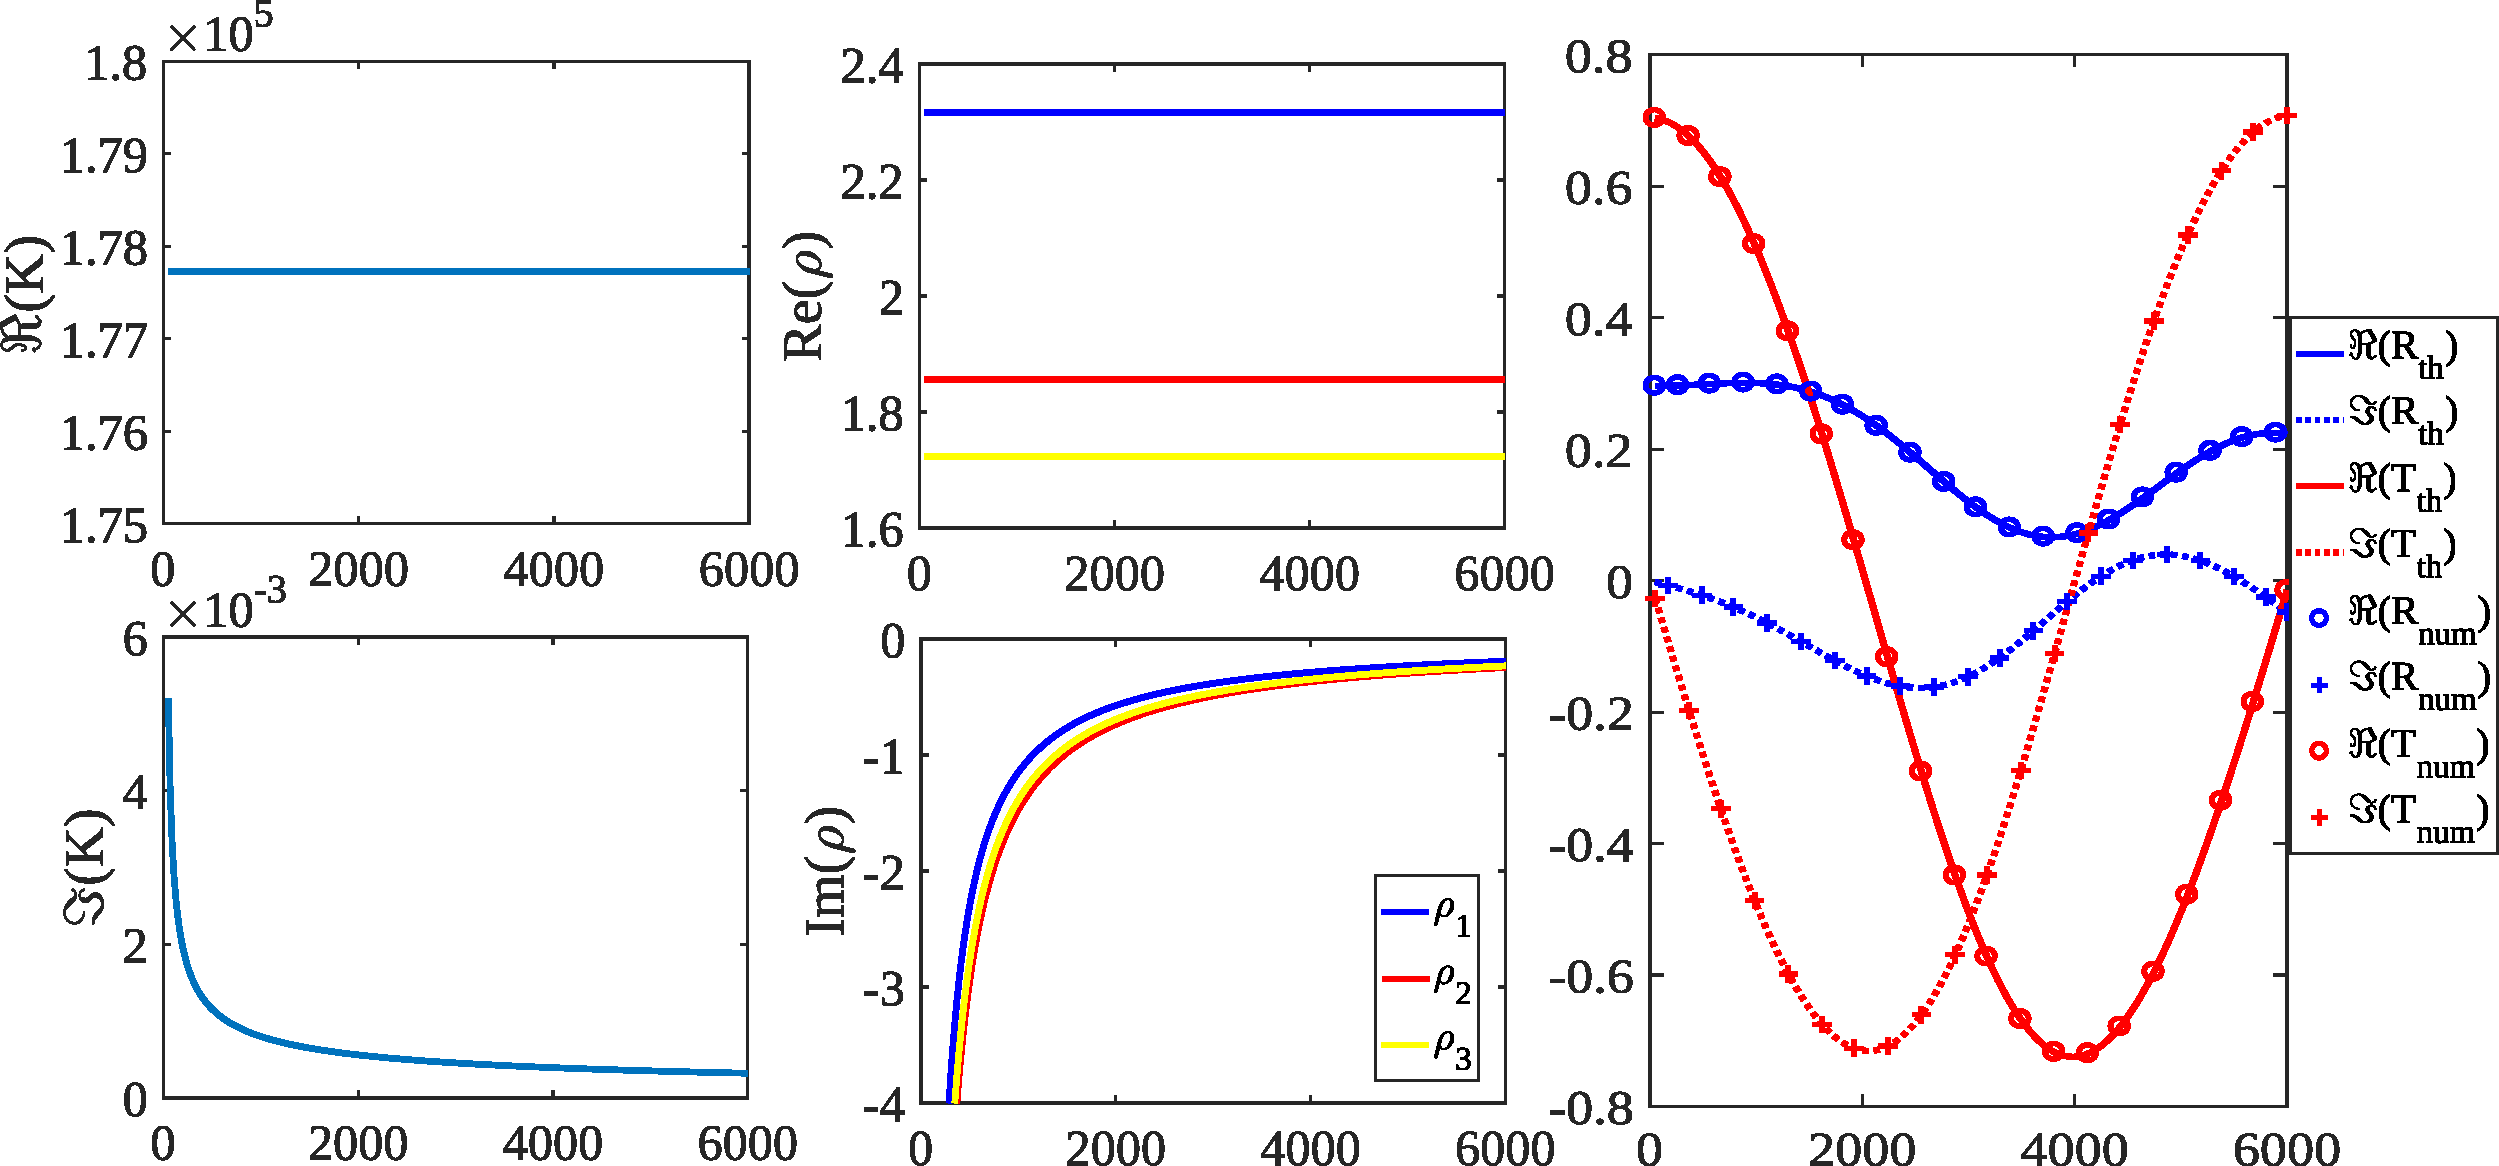
\includegraphics[scale=0.4]{RT_num_th.pdf}
    \caption{ Coefficients de transmission et réflexion (colonne 3) obtenus par un calcul numérique et analytique de la matrice de transfère $Tr$ du milieu fluide équivalent. Les paramètres du fluide équivalent sont le bulk modulus complexe (colonne 1) et les trois densités principales complexes (colonne 2). Une concordance parfaite est observée pour les R et T calculés numériquement et analytiquement.}
    \label{RT_comp}
\end{figure}
    
    Un concordance parfaite est obtenue pour les coefficients R et T en incidence normale, pour toutes les fréquences du domaine étudié. La validation des expressions (\ref{Transmission}) et (\ref{Reflexion}) est donc concluante. 

%%%%%%%%%%%%%%%%%%%%%%%%%%%%%%%%%%%%%%%%%%%%%%%%%%%%%%%%%%%%%%%%%%%%%%%%%%%%%%%%%%%%%%%%%%%%%%%%%%%%%%%%%%%%%%%%%%%%%%%%%%%%%%%%%%%%%%%%%%%%%%%%%%%%%%%%%%%%%%%%%%%%%%%%%%%%%%%%%%%%%%%%%%%%%%%%%%%%%%%%%%%%%%%%%%%%%%%%%%%%%%%%%%%%%%%%%%%%%%%%%%%%%%%%%%%%%%%%%%%%
\chapter{Problème inverse : Détermination de la matrice de densité $\bar{\bar{\rho}}$ et du Bulk modulus équivalent $\tilde{K}$}
\label{Ch_Inv}
	A ce stade de l'étude du problème, il a été possible d'obtenir la matrice de transfert $Tr$ de la couche fluide équivalente, et en appliquant des conditions initiales, les coefficients de réflexions et transmissions ont pu être déterminés.
	
	Il est donc possible maintenant de développer une méthode inverse, visant à déterminer les paramètres du milieux fluide équivalent, soit la matrice de densités complexe $\bar{\bar{\rho}}$ et le bulk modulus $K$, à partir de couple de coefficients de réflexion et transmission R/T connus pour différents angles d'incidence.
	La méthode développée permet d'identifier les sept paramètres caractérisant le fluide, six densités complexes et un bulk modulus, à partir de six couples R/T, soit douze informations. A première vue, la méthode est surdimensionnée avec douze informations pour six inconnues, mais en regardant plus en détail, il est possible de voir que les six couples de données donnent l'information sur les six densités, ainsi que six informations redondantes sur le bulk modulus. Le surdimensionement vient donc des six informations sur le bulk modulus contenues dans chaque couple de données. 
    
    Il est important de noter ici que la longueur L de la couche fluide est supposée déterminée par une autre méthode précédemment, et que dans la méthode proposée, L est considérée comme connue.
    
    La méthode peut se décrire en plusieurs étapes, dans un premier temps le bulk modulus est déterminé en incidence normale, puis les termes de phases sont identifiés par une variation de phase du coefficient de transmission T le long des directions $x_1$ et $x_2$. Finalement, pouvant identifier l'impédance $Z_3$ caractérisant la propagation dans la couche fluide, les densité sont déterminées.
    
\section{Rappel du problème de propagation dans la couche fluide}
\label{Ch_Inv_S_Pb}
    Il est ici rappelé  les paramètres (\ref{Ktild}), (\ref{rho3tild}), (\ref{q1}) et (\ref{q2})  de la couche fluide équivalente:
    \begin{align*}
	    &\bar{\bar{\rho}}=\begin{pmatrix} \rho_1 & \rho_{12} & \rho_{13} \\ \rho_{12} & \rho_2 & \rho_{23} \\ \rho_{13} & \rho_{23} & \rho_3 \end{pmatrix},\\
        &\bar{\bar{A}}=\begin{pmatrix} i \tilde{q} & i \omega \tilde{\rho_3} \\ \frac{i \omega}{\tilde{K}} & i \tilde{q} \end{pmatrix},\\
	    &\tilde{K}=\frac{K}{[1-\frac{\rho_{33}}{\rho_{11}\rho_{22}-\rho_{12}^2}(\frac{k_1}{k_3^{(i)}})^2(\rho_{22}-\rho_{12}\frac{k_2}{k_1})-\frac{\rho_{33}}{\rho_{11}\rho_{22}-\rho_{12}^2}(\frac{k_2}{k_3^{(i)}})^2(\rho_{11}-\rho_{12}\frac{k_1}{k_2})]},\\
        &\tilde{\rho_3}=\rho_{33}[1-\frac{\rho_{13}}{\rho_{11}\rho_{22}-\rho_{12}^2}(\frac{k_1^{(i)}}{k_3^{(i)}})^2(\rho_{22}-\rho_{12}(\frac{k_2^{(i)}}{k_1^{(i)}})^2)-\frac{\rho_{23}}{\rho_{11}\rho_{22}-\rho_{12}^2}(\frac{k_2^{(i)}}{k_3^{(i)}})^2(\rho_{11}-\rho_{12}(\frac{k_1^{(i)}}{k_2^{(i)}})^2)], \\
        &\tilde{q}=q_1+q_2,\\
	    &q_{1}=\frac{\rho_{22}\rho_{13}-\rho_{12}\rho_{23}}{\rho_{11}\rho_{22}-\rho_{12}^2}k_1,\\
        &q_{2}= \frac{\rho_{11}\rho_{23}-\rho_{12}\rho_{13}}{\rho_{11}\rho_{22}-\rho_{12}^2}k_2.
    \end{align*}
    
    De même, les projections du nombre d'onde [(\ref{k1}):(\ref{k3})] sont :
    \begin{align*}
    &k_1=-k_0 sin(\theta) cos(\phi), \\
    &k_2=-k_0 sin(\theta) sin(\phi), \\
    &k_3= -k_0 cos(\theta).
    \end{align*}
          
     
\section{Impédance effective $Z_3$ et nombre d'onde effectif $k_{33}$}
\label{Ch_Inv_S_Z3}
Afin de pouvoir mettre en place la méthode inverse, il faut dans un premier temps définir une variable permettent de connaître la propagation dans le milieu fluide. D'après l'équation (\ref{Eq_Prop}), deux paramètres peuvent être utilisés, l'impédance $Z_3$ et le nombre d'onde $k_{33}$, il est donc proposé ici d'exprimer ces deux termes en fonction de R et T.
    
    Avec l'équation (\ref{eqDif_tmp}), il est possible d'écrire les deux équations suivantes :
    \begin{align}
        &e^{i k_{33}L}=\frac{(p_0-Z_3v_0)}{(p_L-Z_3v_L)}e^{i\tilde{q}L},\label{Eq_Prop_tmp2}\\
        &e^{-i k_{33}L}=\frac{(p_0+Z_3v_0)}{(p_L+Z_3v_L)}e^{i\tilde{q}L},\label{Eq_Prop_tmp3}
    \end{align}
    de ces deux expressions, il est possible de déterminer les deux paramètres $Z_3$ et $k_{33}$.
    Dans un premier temps, en écrivant le produit (\ref{Eq_Prop_tmp2})x(\ref{Eq_Prop_tmp3}), il est possible d'annuler les termes en $k_{33}$ et il vient : 
    \begin{align}
    Z_3^2=\frac{p_0^2-p_L^2e^{-2i\tilde{q}L}}{v_0^2-v_L^2e^{-2i\tilde{q}L}}=\frac{T^2e^{2iq_1L}-(1+R)^2}{T^2e^{2i\tilde{q}L}-(1-R)^2}Z^2\label{Z3_tmp}
    \end{align}
    Il est donc possible d'exprimer l'impédance effective $Z_3$ en fonction de R et de T, Z, ainsi que du terme de phase $\tilde{q}$. Les trois premiers termes R, T et Z sont connus dans notre problème, connaissant l'excitation et les coefficients R et T mesurés. En revanche $\tilde{q}$, n'est pas déterminé à ce stade du problème, et en reprenant son expression $\tilde{q}=q_1+q_2$, il n'est connu que en incidence normale où il est nul. L'impédance $Z_3$ n'est donc déterminée pour le moment que en incidence normale. Finalement, il est défini ici une fonction $F(R,T,\tilde{q})$, permettant d'obtenir l'impédance $Z_3$ à partir de R et T comme :
    \begin{align}
    &Z_3=F(R,T,\tilde{q})Z,\label{Z3}\\
    &F(R,T,\tilde{q})=\sqrt{\frac{T^2e^{2i\tilde{q}l}-(1+R)^2}{T^2e^{2i\tilde{q}L}-(1-R)^2}}.\label{F(R,T,q)}
    \end{align}

    
    En reprenant l'expression (\ref{Eq_Prop_tmp2}), il est possible d'exprimer $k_{33}$. $\xi$ est posé telle que $\xi=\frac{(p_0-Z_3v_0)}{(p_L-Z_3v_L)}e^{i\tilde{q}L}=|\xi|e^{i\psi}$. De plus il est possible d'écrire, en rappelant que $k_{33}$ est complexe, $k_{33}=\Re(k_{33})+i\ \Im(k_{33})$, il est finalement possible d'écrire :
     \begin{align}
        k_{33}=\frac{\psi-i\ ln(|\xi|)}{L}\label{k_{33}}.
    \end{align}
    Le nombre d'onde effectif $k_{33}$ peut, de la même façon que $z_3$, être obtenu en incidence normale mais n'est pas défini pour tous les angles d'incidence.
    
\section{Bulk modulus équivalent $\tilde{K}$}
\label{Ch_Inv_S_K}
Afin de pouvoir identifier les densités du fluide équivalent, il est nécessaire de connaître l'impédance $Z_3$  et le bulk modulus $K$, il est ici proposé de déterminer $K$.
    
    Comme dit précédemment, l'information de $K$ est contenue pour chaque couple R/T, et plus précisément dans les paramètres $Z_3$ et $k_{33}$ qui nous intéressent en incidence normale.
    
    Par définition l'on peut écrire :
    \begin{align}
        Z_3=\tilde{\rho_3}c_{33}=\sqrt{\tilde{\rho_3}\tilde{K}},\label{Z3_tmp2}\\
        k_{33}=\frac{\omega}{c_{33}}=\sqrt{\frac{\tilde{\rho_3}}{\tilde{K}}}\label{k33_tmp}
    \end{align}
    Sachant que l'expression de $\tilde{K}$ (\ref{Ktild}) devient en incidence normale $\tilde{K}=K$, il est possible d'écrire par simple produit ou division de (\ref{Z3_tmp2}) et (\ref{k33_tmp}) :
    \begin{align}
        K=\frac{Z_3}{k_{33}}\omega|^{\theta=0}_{\phi=0},\label{K}\\
        \tilde{\rho_3}=\frac{Z_3k_{33}}{\omega}|^{\theta=0}_{\phi=0}.\label{rho3tild_id}
    \end{align}
    
    $K$ et $\tilde{\rho_3}$ peuvent donc être identifiés en incidence normale.

\section{Termes de phase $\tilde{q}=q_1+q_2$}
\label{Ch_Inv_S_q}
    Afin de connaître $Z_3$ pour chaque angle d'incidence, et donc de pouvoir déterminer la matrice densité $\bar{\bar{\rho}}$, le terme de phase $\tilde{q}$ doit être identifié. $\tilde{q}$ correspond à une variation de la phase de l'onde transmise, due à un couplage induit par les densités $\rho_{13}$ et $\rho_{23}$. Afin d'observer la variation de phase produite par $\tilde{q}$, il est possible d'étudier le coefficient de transmission pour deux ondes incidentes, de même angle azimutal $\phi$ et d'élévation $\theta $ opposée, ainsi pour deux ondes incidentes le long d'une même direction, un déphasage de transmission sera observé et l'on pourra remonter au terme de phase $\tilde{q}$.
    
    Du point de vue mathématique, cela peut s'expliquer en s'intéressant à l'expression (\ref{Transmission}) du coefficient de transmission. Pour un angle azimutal $\phi$ fixé, si l'on considère deux angles d'incidence opposés $\pm \theta$, l'expression ne change que par le terme en $\tilde{q}$. $k_{33}$ et $Z_3$ varient avec l'angle d'incidence de part $\tilde{K}$, or d'après l'expression (\ref{Ktild}), il est possible de montrer $\tilde{K}|^{+\theta}_{\phi}=\tilde{K}|^{-\theta}_{\phi}$. De plus l'impédance Z dépend d'une fonction paire de l'élévation $\theta$, il est donc montré que la variation du coefficient de transmission T ne dépend que du terme de phase $\tilde{q}$.
    
    Si l'on étudie l'expression de $q_1$ (\ref{q1}) et de $q_2$ (\ref{q2}), il est possible de choisir deux couples d'angle d'incidence $\theta$ et $\phi$ adéquates, afin d'isoler l'influence de soit $q_1$, soit $q_2$, dans le terme de phase $\tilde{q}$. Afin d'isoler le terme $q_1$, il est proposé de prendre deux angles d'incidences le long de l'axe $x_1$, soit un angle azimutal de $\phi=0$, d'où $k_2=q_2=0$, de plus pour deux angles d'élévation opposés $\theta=\pm \frac{\pi}{6}$, il est possible d'écrire $q_1|^{\theta=\frac{\pi}{6}}_{\phi=0}=-q_1|^{\theta=\frac{-\pi}{6}}_{\phi=0}$. De même pour isoler $q_2$, il est possible de prendre deux angles d'incidence opposés le long de $x_2$, tels que $\theta=\pm \frac{\pi}{6}$ et $\phi=\frac{\pi}{2}$.
    
    Il est ici défini les deux termes $q_1^{(0)}$ et $q_2^{(0)}$ correspondant aux termes $q_1$ et $q_2$ sans projection du nombre d'onde incident $k^{(0)}$, tels que :
    \begin{align}
            &q_1^{(0)}=\frac{\rho_2\rho_{13}-\rho_{12}\rho_{23}}{\rho_1\rho_2-\rho_{12}^2}k^{(0)},\label{q1,0}\\
        &q_2^{(0)}=\frac{\rho_1\rho_{23}-\rho_{12}\rho_{13}}{\rho_1\rho_2-\rho_{12}^2}k^{(0)}.\label{q2,0}
    \end{align}
    
    Considérant l'expression (\ref{Transmission}), le rapport de coefficient de transmission pour les deux couples choisis s'écrit :
    \begin{align}
     e^{iq_1^{(0)}L}=\frac{T^{\theta=\frac{\pi}{6}}_{\phi=0}}{T^{\theta=\frac{-\pi}{6}}_{\phi=0}},\ e^{iq_2^{(0)}L}=\frac{T^{\theta=\frac{\pi}{6}}_{\phi=\frac{-\pi}{2}}}{T^{\theta=\frac{-\pi}{6}}_{\phi=\frac{-\pi}{2}}},
    \end{align}
    et utilisant la même méthode que pour $k_{33}$, il est possible d'identifier $q_1^{(0)}$ et $q_2^{(0)}$ et donc $q_1$ et $q_2$.
    
\section{Identification des densités du fluide équivalent}    
\label{Ch_Inv_S_rho}
\subsection{Système d'équation}
\label{Ch_Inv_S_rho_SS_eq}
    Maintenant que le bulk modulus $K$ est connu ainsi que le terme de phase $\tilde{q}$, l'impédance effective $Z_3$ est connu pour tout les angles d'incidence, il est proposé d'identifier les différentes densités en utilisant les données connues à travers $Z_3$.
    
	L'impédance est ici réécrite de façon à mettre en évidence les différents paramètres à identifier, c'est-à-dire les densités complexes. En posant $\tilde{K}=\frac{K}{\alpha}$, il est possible d'exprimer $Z_3$, en développant l'expression (\ref{Ktild}), comme :
	\begin{align}
        &Z_3=\sqrt{\tilde{\rho_3}\tilde{K}}=\sqrt{\frac{\tilde{\rho_3}K}{\alpha}},
        \intertext{avec :}
        &\alpha=1-\frac{K}{\omega^2}\frac{\rho_2 k_1^2+\rho_1 k_2^2-2\rho_{12}k_1k_2}{\rho_1\rho_2-\rho_{12}^2}.
    \end{align}
    Il vient donc :
    \begin{align}
        \alpha=\frac{\tilde{\rho_3}K}{Z_3^2},
    \end{align}
    et il est posé l'équation suivante pour l'identification des densités :
     \begin{align}
        \frac{K}{\omega^2}\frac{\rho_2k_1^2 +\rho_1k_2^2-2\rho_{12}k_1k_2}{\rho_1\rho_2-\rho_{12}^2}=1-\frac{\tilde{\rho_3}K}{Z_3^2}.\label{Eq_res}
    \end{align}
    
    Afin de simplifier la résolution du problème, $\gamma$ est ci-dessous défini et la notation indicielle des angles d'incidence est mise en place :
    
    \begin{align}
        &\gamma=1-\frac{\tilde{\rho_3}K}{Z_3^2},\label{gamma}\\
        &X^{(x)}_{(y)}=X|^{\theta=x}_{\phi=y}.\label{notation_angle}
    \end{align}
    
\subsection{Densités $\rho_1$, $\rho_2$ et $\rho_{12}$}
\label{Ch_Inv_S_rho_SS_rho1/2/12}
    L'expression (\ref{Eq_res}) fait apparaître trois densités à déterminer, il faut donc donc trois couples R/T à des angles d'incidence différents pour pouvoir résoudre un système de trois équations à trois inconnues, et donc identifier les trois densités $\rho_1$, $\rho_2$ et $\rho_{12}$.
    Considérant les projection du nombre d'onde incident $k^{(0)}$ mises en jeu dans l'équation (\ref{Eq_res}), les trois angles d'incidence peuvent être choisis afin d'isoler l'influence de chacune des densités. En reprenant deux des angles d'incidence utilisés pour déterminer $\tilde{q}$, $\theta=\frac{\pi}{6}$ et $\phi=0$ ainsi que $\theta=\frac{\pi}{6}$ et $\phi=\frac{\pi}{2}$, il est possible d'annuler soit $k_1$ soit $k_2$. De plus si un troisième angle d'incidence, dit "oblique", est pris tel que $k_1\ne 0$ et $k_2\ne 0$, avec la même projection du nombre, dans notre cas $\theta=\frac{\pi}{4}$ et $\phi=\frac{\pi}{4}$, il est possible d'écrire :
    \begin{align}
        k=k_1|^{(\frac{\pi}{6})}_{(0)}=k_2|^{(\frac{\pi}{6})}_{(\frac{\pi}{2})}=k_1|^{(\frac{\pi}{4})}_{(\frac{\pi}{4})}=k_2|^{(\frac{\pi}{4})}_{(\frac{\pi}{4})}=\frac{1}{2}k^{(0)}.
    \end{align}
    
    L'expression (\ref{Eq_res}) pour les trois angles d'incidence se réécrit :
        \begin{align}
    &\frac{K}{\omega^2}\frac{\rho_2}{\rho_1\rho_2-\rho_{12}^2}k^2=\gamma^{(\frac{\pi}{6})}_{(0)}\label{Comp_1},\\ &\frac{K}{\omega^2}\frac{\rho_1}{\rho_1\rho_2-\rho_{12}^2}k^2=\gamma^{(\frac{\pi}{6})}_{(\frac{\pi}{2})}\label{Comp_2},\\ &\frac{K}{\omega^2}\frac{\rho_1+\rho_2-2\rho_{12}}{\rho_1\rho_2-\rho_{12}^2}k^2=\gamma^{(\frac{\pi}{4})}_{(\frac{\pi}{4})}\label{Comp_3}.
    \end{align}

    Les expressions [(\ref{Comp_1}):(\ref{Comp_3})] permettent d'écrire les rapports de densité suivants, et ainsi de déterminer un ratio $X_i$ entre ces densités :
    \begin{align}
    &\frac{(\ref{Comp_2})}{(\ref{Comp_1})} :\ \frac{\rho_1}{\rho_2}=\frac{\gamma|^{(\frac{\pi}{6})}_{(0)}}{\gamma|^{(\frac{\pi}{6})}_{(\frac{\pi}{2})}}=X_1,\label{Comp_rho2_rho1} \\
    &\frac{(\ref{Comp_1})+(\ref{Comp_2})-(\ref{Comp_3})}{(\ref{Comp_2})} :\ \frac{\rho_{12}}{\rho_1}=\frac{1}{2}\frac{\gamma|^{(\frac{\pi}{6})}_{(0)}+\gamma|^{(\frac{\pi}{6})}_{(\frac{\pi}{2})}-\gamma|^{(\frac{\pi}{4})}_{(\frac{\pi}{4})}}{\gamma|^{(\frac{\pi}{6})}_{(\frac{\pi}{2})}}=X_2,\label{Comp_rho12_rho1} \\
    &\frac{(\ref{Comp_1})+(\ref{Comp_2})-(\ref{Comp_3})}{(\ref{Comp_1})} :\ \frac{\rho_{12}}{\rho_2}=\frac{1}{2}\frac{\gamma|^{(\frac{\pi}{6})}_{(0)}+\gamma|^{(\frac{\pi}{6})}_{(\frac{\pi}{2})}-\gamma|^{(\frac{\pi}{4})}_{(\frac{\pi}{4})}}{\gamma|^{(\frac{\pi}{6})}_{(0)}}=X_3.\label{Comp_rho12_rho2}
    \end{align}
    
    En introduisant ces rapports de densité dans l'une des trois équations [(\ref{Comp_1}):(\ref{Comp_3})], ici (\ref{Comp_2}), il vient : 
    \begin{align}
    &\rho_2=\frac{X_1}{(X_1-X_3^2)\gamma|^{(\frac{\pi}{6})}_{(\frac{\pi}{2})}},\label{Comp_rho2}\\
    &\rho_1=X_1\rho_2,\label{Comp_rho1}\\
    &\rho_{12}=X_3\rho_2.\label{Comp_rho12}
    \end{align}
    
    Finalement, en développant les ratio $X_i$ dans les expressions [(\ref{Comp_rho1}):(\ref{Comp_rho12})], il est possible de déterminer les trois densités $\rho_1$, $\rho_2$ et $\rho_{12}$ :
    \begin{align}
        &\rho_1=\frac{\gamma^{(\frac{\pi}{6})}_{(\frac{\pi}{2})}}{\gamma^{(\frac{\pi}{6})}_{(0)}\gamma^{(\frac{\pi}{6})}_{(\frac{\pi}{2})}-\frac{1}{4}(\gamma^{(\frac{\pi}{6})}_{(0)}+\gamma^{(\frac{\pi}{6})}_{(\frac{\pi}{2})}-\gamma^{(\frac{\pi}{4})}_{(\frac{\pi}{4})})^2},\label{rho1}\\
        &\rho_2=\frac{\gamma^{(\frac{\pi}{6})}_{(0)}}{\gamma^{(\frac{\pi}{6})}_{(0)}\gamma^{(\frac{\pi}{6})}_{(\frac{\pi}{2})}-\frac{1}{4}(\gamma^{(\frac{\pi}{6})}_{(0)}+\gamma^{(\frac{\pi}{6})}_{(\frac{\pi}{2})}-\gamma^{(\frac{\pi}{4})}_{(\frac{\pi}{4})})^2},\label{rho2}\\
        &\rho_{12}=\frac{\gamma^{(\frac{\pi}{6})}_{(0)}+\gamma^{(\frac{\pi}{6})}_{(\frac{\pi}{2})}-\gamma^{(\frac{\pi}{4})}_{(\frac{\pi}{4})}}{\gamma^{(\frac{\pi}{6})}_{(0)}\gamma^{(\frac{\pi}{6})}_{(\frac{\pi}{2})}-\frac{1}{4}(\gamma^{(\frac{\pi}{6})}_{(0)}+\gamma^{(\frac{\pi}{6})}_{(\frac{\pi}{2})}-\gamma^{(\frac{\pi}{4})}_{(\frac{\pi}{4})})^2}.\label{rho12}
    \end{align}

\subsection{Densités $\rho_{13}$, $\rho_{23}$ et $\rho_3$}
\label{Ch_Inv_S_rho_SS_rho13/23/3}
    Les trois densités $\rho_{13}$, $\rho_{23}$ et $\rho_3$ restent à déterminer. L'identification peut être fait à partir des paramètres déjà connus, $q_1^{(0)}$, $q_2^{(0)}$ et $\tilde{\rho_3}$, les trois densités étant les seules inconnues restantes.
    
    En rappelant les expressions (\ref{q1,0}) et (\ref{q2,0}) de $q_1^{(0)}$ et $q_2^{(0)}$, il vient le système de deux équations à deux inconnues suivant :
    \begin{align*}
    &q_1^{(0)}=\frac{\rho_1\rho_{23}-\rho_{12}\rho_{13}}{\rho_1\rho_2-\rho_{12}^2}k^{(0)},\\
    &q_2^{(0)}=\frac{\rho_2\rho_{13}-\rho_{12}\rho_{23}}{\rho_1\rho_2-\rho_{12}^2}k^{(0)}.
    \end{align*}
    La résolution du système amène à :
    \begin{align*}
    \rho_{13}=\frac{\rho_1q_1^{(0)}+\rho_{12}q_2^{(0)}}{k^{(0)}},\\
    \rho_{23}=\frac{\rho_2q_2^{(0)}+\rho_{12}q_1^{(0)}}{k^{(0)}}.
    \end{align*}

    De plus d'après l'expression de $\tilde{\rho_3}$ (\ref{rho3tild}), il vient :
    \begin{align}
    \rho_3=\tilde{\rho_3}+\frac{\rho_{13}(\rho_2\rho_{13}-\rho_{12}\rho_{23})+\rho_{23}(\rho_1\rho_{23}-\rho_{12}\rho_{13})}{\rho_1\rho_2-\rho_{12}^2}.
    \end{align}
    
\section{Conclusion}
\label{Ch_Inv_S_Conc}
    Une méthode inverse a pu être développée pour retrouver les paramètres du fluide équivalent à partir de la longueur de la couche fluide selon $x_3$ et de six couples R/T pour six angles d'incidence différents, les six angles étant :\\
    \begin{tabular}{||m{3cm}||m{3cm}|m{3cm}|m{3cm}|m{3cm}|}
         \hline
         $\theta (rad)$ & 0 & $\pm\frac{\pi}{6}$ & $\pm\frac{\pi}{6}$ & $\frac{\pi}{4}$ \\ \hline 
          $\phi (rad)$ & 0 & 0 & $\frac{\pi}{2}$ & $\frac{\pi}{4}$
          \\ \hline
    \end{tabular}\\
    
    La méthode peut se diviser en cinq étapes de résolution listées ci-dessous 
    \begin{itemize}
        \item 1) Détermination du bulk modulus et de $\tilde{\rho_3}$ en incidence normale
        \item 2) Détermination des deux termes de phases $q_1$ et $q_1$ pour respectivement deux angles d'incidence opposés le long de $x_1$ et $x_2$
        \item 3) Identification des trois densités du plan $\rho_1$, $\rho_2$ et $\rho_{12}$ avec trois angles d'incidence selon $x_1$, $x_2$ et médian.
        \item 4) Identification des densités $\rho_{13}$ et $\rho_{23}$ à partir de $q_1$ et $q_2$.
        \item 5) Identification de $\rho_3$ avec $\tilde{\rho_3}$
    \end{itemize}
    
    La méthode proposée permet de retrouver le bulk modulus et la matrice de densité complexe de la couche fluide équivalente, autrement dit, quelque soit la rotation des directions principales du fluide, des paramètres peuvent être identifiés. Sans aucune connaissance de la géométrie du milieu, il est donc possible de retrouver ses paramètres, avec rotation des directions principales, et dans ses directions principales en résolvant une simple problème au valeur propre.  
    
    
    
    
%%%%%%%%%%%%%%%%%%%%%%%%%%%%%%%%%%%%%%%%%%%%%%%%%%%%%%%%%%%%%%%%%%%%%%%%%%%%%%%%%%%%%%%%%%%%%%%%%%%%%%%%%%%%%%%%%%%%%%%%%%%%%%%%%%
\chapter{Résultats}
\label{Ch_Res}
  \begin{figure}[ht!]
        \centering
        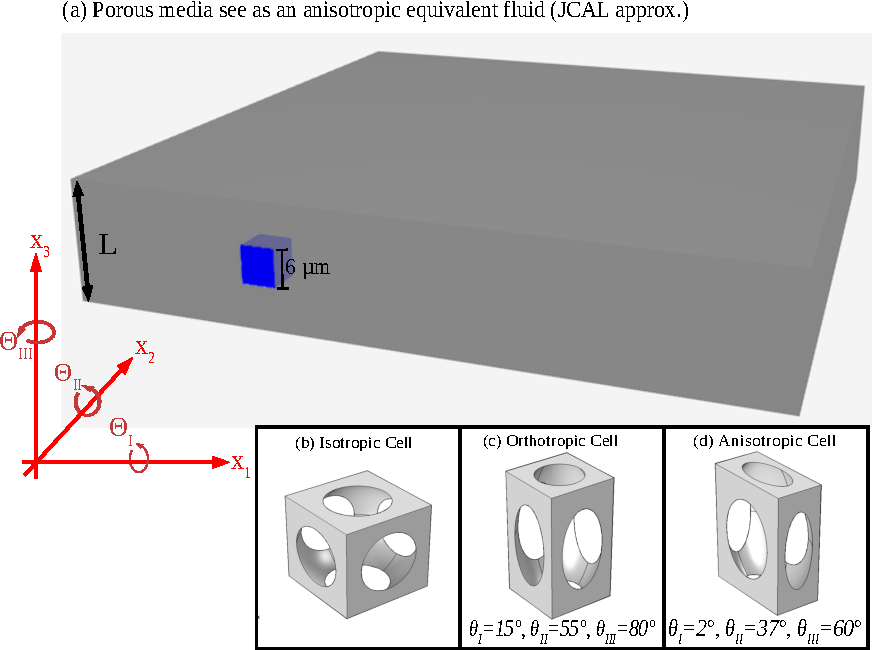
\includegraphics{Material_2.pdf}
        \caption{Couche de matériau poreux constituée de pores ellipsoïdes homogénéisés par le modèle JCAL (citation). La couche est de largeur L=5cm et est supposée infinie dans le plan $x_1x_2$. Trois cas différents sont utilisés avec trois cellules ellipsoïdes différentes, une isotrope (b), une orthotrope (c) et une anisotrope (d). Pour les deux dernières, les directions du matériaux sont considérées comme ayant subi une rotation. Les trois angles d'Euler "ZYX", autour de $x_1$, $x_2$ et $x_3$ sont notés sous la cellule. }
        \label{Porous_Mat}
    \end{figure}

    La méthode ayant été décrite dans la partie \ref{Ch_Inv}, il est maintenant proposé de faire une validation numérique de la méthode à partir d'un matériau poreux. Le matériau poreux, décrit sur la figure (\ref{Porous_Mat}), de longueur L=5cm selon $x_3$ et infinie dans le plan $x_1x_2$, est constitué de cellules ellipsoïdales de différentes formes. Trois cas sont étudiés ici, avec une cellule isotrope, une cellule orthotrope et une cellule anisotrope. Une rotation des directions principales du fluide équivalent anisotrope est faite selon les trois angles d'Euler en configuration "ZYX" autour de $x_1$, $x_2$ et $x_3$. La rotation du milieux est décrites dans l'annexes A (Ref). L'homogénéisation du poreux étant faite avant la rotation du milieu, aucune modification n'est prise en compte dans le cas isotrope. Les trois angles de rotation du cas orthotrope sont $\theta_I=15\textdegree$, $\theta_{III}=55\textdegree$ et $\theta_{II}=80\textdegree$, et dans le cas anisotrope $\theta_I=2\textdegree$, $\theta_{II}=37\textdegree$ et $\theta_{III}=60\textdegree$.
    
    \begin{figure}[ht!]
        \centering
        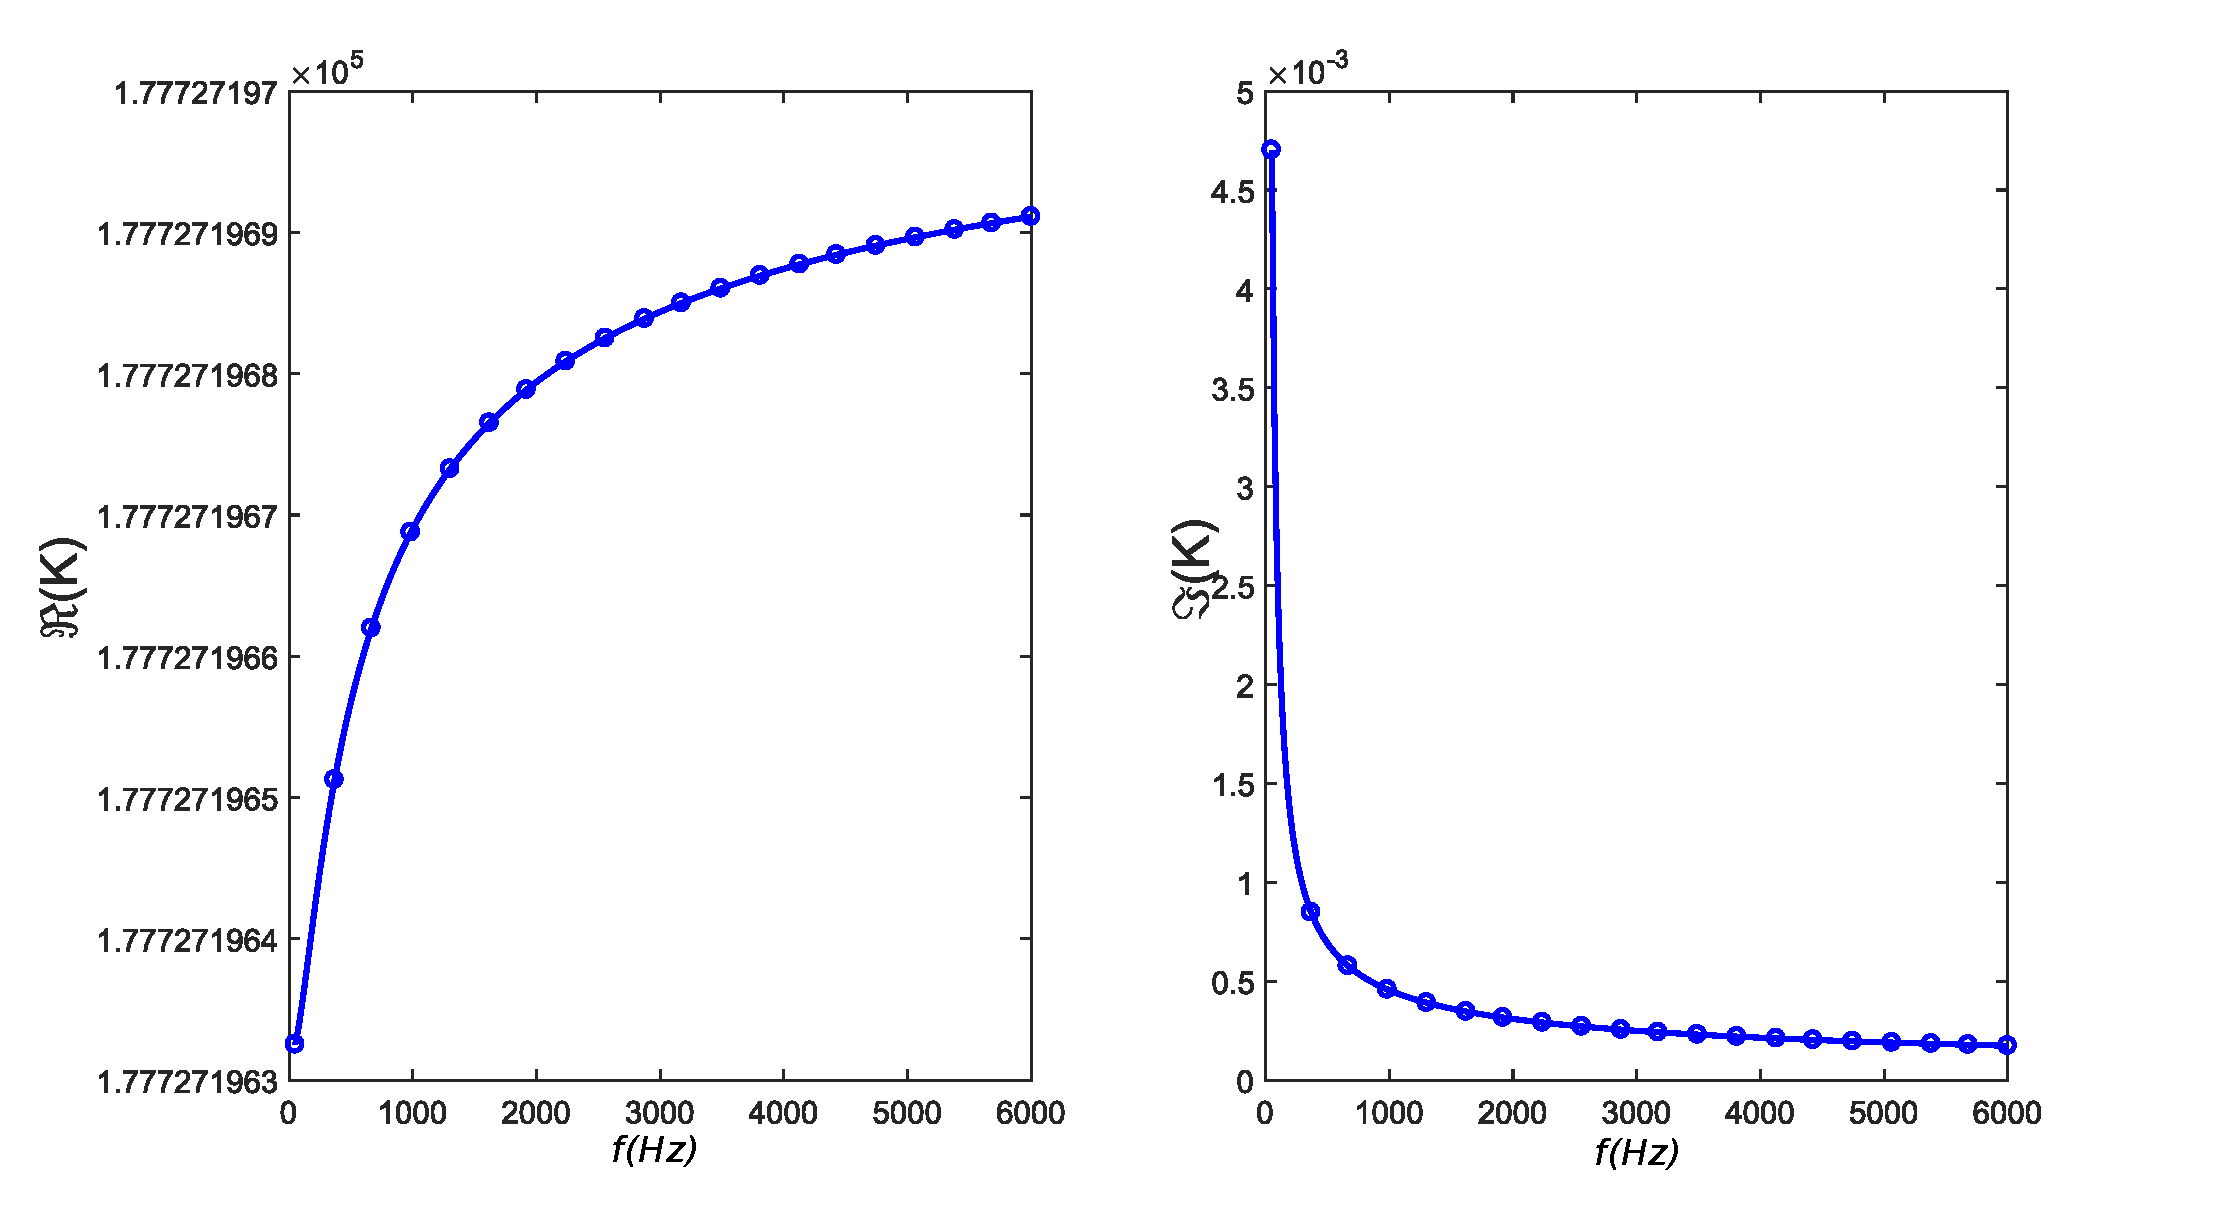
\includegraphics[scale=0.45]{Bulk.pdf}
        \caption{Bulk modulus reconstruit (ligne continue) et théorique(marqueurs rond), dans le cas sans bruit, pour les trois types de matériaux poreux homogénéisés, isotrope, orthotrope et anisotrope.}
        \label{bulk}
    \end{figure}
    
    Pour les trois cas, les six couples R/T sont obtenus avec un modèle de propagation fluide pour les six angles d'incidence nécessaires à la méthode. Les paramètres des trois différents fluides (isotrope, orthotrope et anisotrope) sont identifiés par la méthode inverse et comparer à ceux du fluide équivalent, dans le cas sans bruit et avec bruit rajouté à R et T. 
    
    Un exemple de signal bruité pour le cas du fluide équivalent anisotrope est représenté sur la figure (\ref{RT_noise}), pour les densités complexes et le bulk également représentés. Les coefficients R et T sont représentés en incidence normale, pour un SNR de 30 dB.  
    
    Dans un premier temps, La reconstruction des paramètres de la couche fluide  est faites dans le cas sans bruit. Ces premier résultat ne permettent pas de valider la méthode, les coefficients R et T étant calculés par le même modèle de propagation dans une couche de fluide équivalent anisotrope que pour celui utilisé pour développer la méthode inverse.  

    Le premiers paramètres reconstruit par la méthode proposée est le bulk modulus en incidence normale, représenté sur la figure (\ref{bulk}) :
    
    Le bulk modulus est parfaitement reconstruit par la méthode, pour les trois types de matériaux. Les R et T étant obtenue pour un même modèle de propagation dans une couche fluide équivalente, il vient donc logiquement que la méthode inverse retrouve les paramètres fidèlement aux paramètres en entrées. 
    
    Les densités complexe sont ensuite identifiées en incidence non-normale, pour les trois cas isotrope, orthotrope et anistrope. Les densités obtenues sont représentés sur la figure (\ref{rho_rot}) :
    \begin{figure}[ht!]
        \centering
        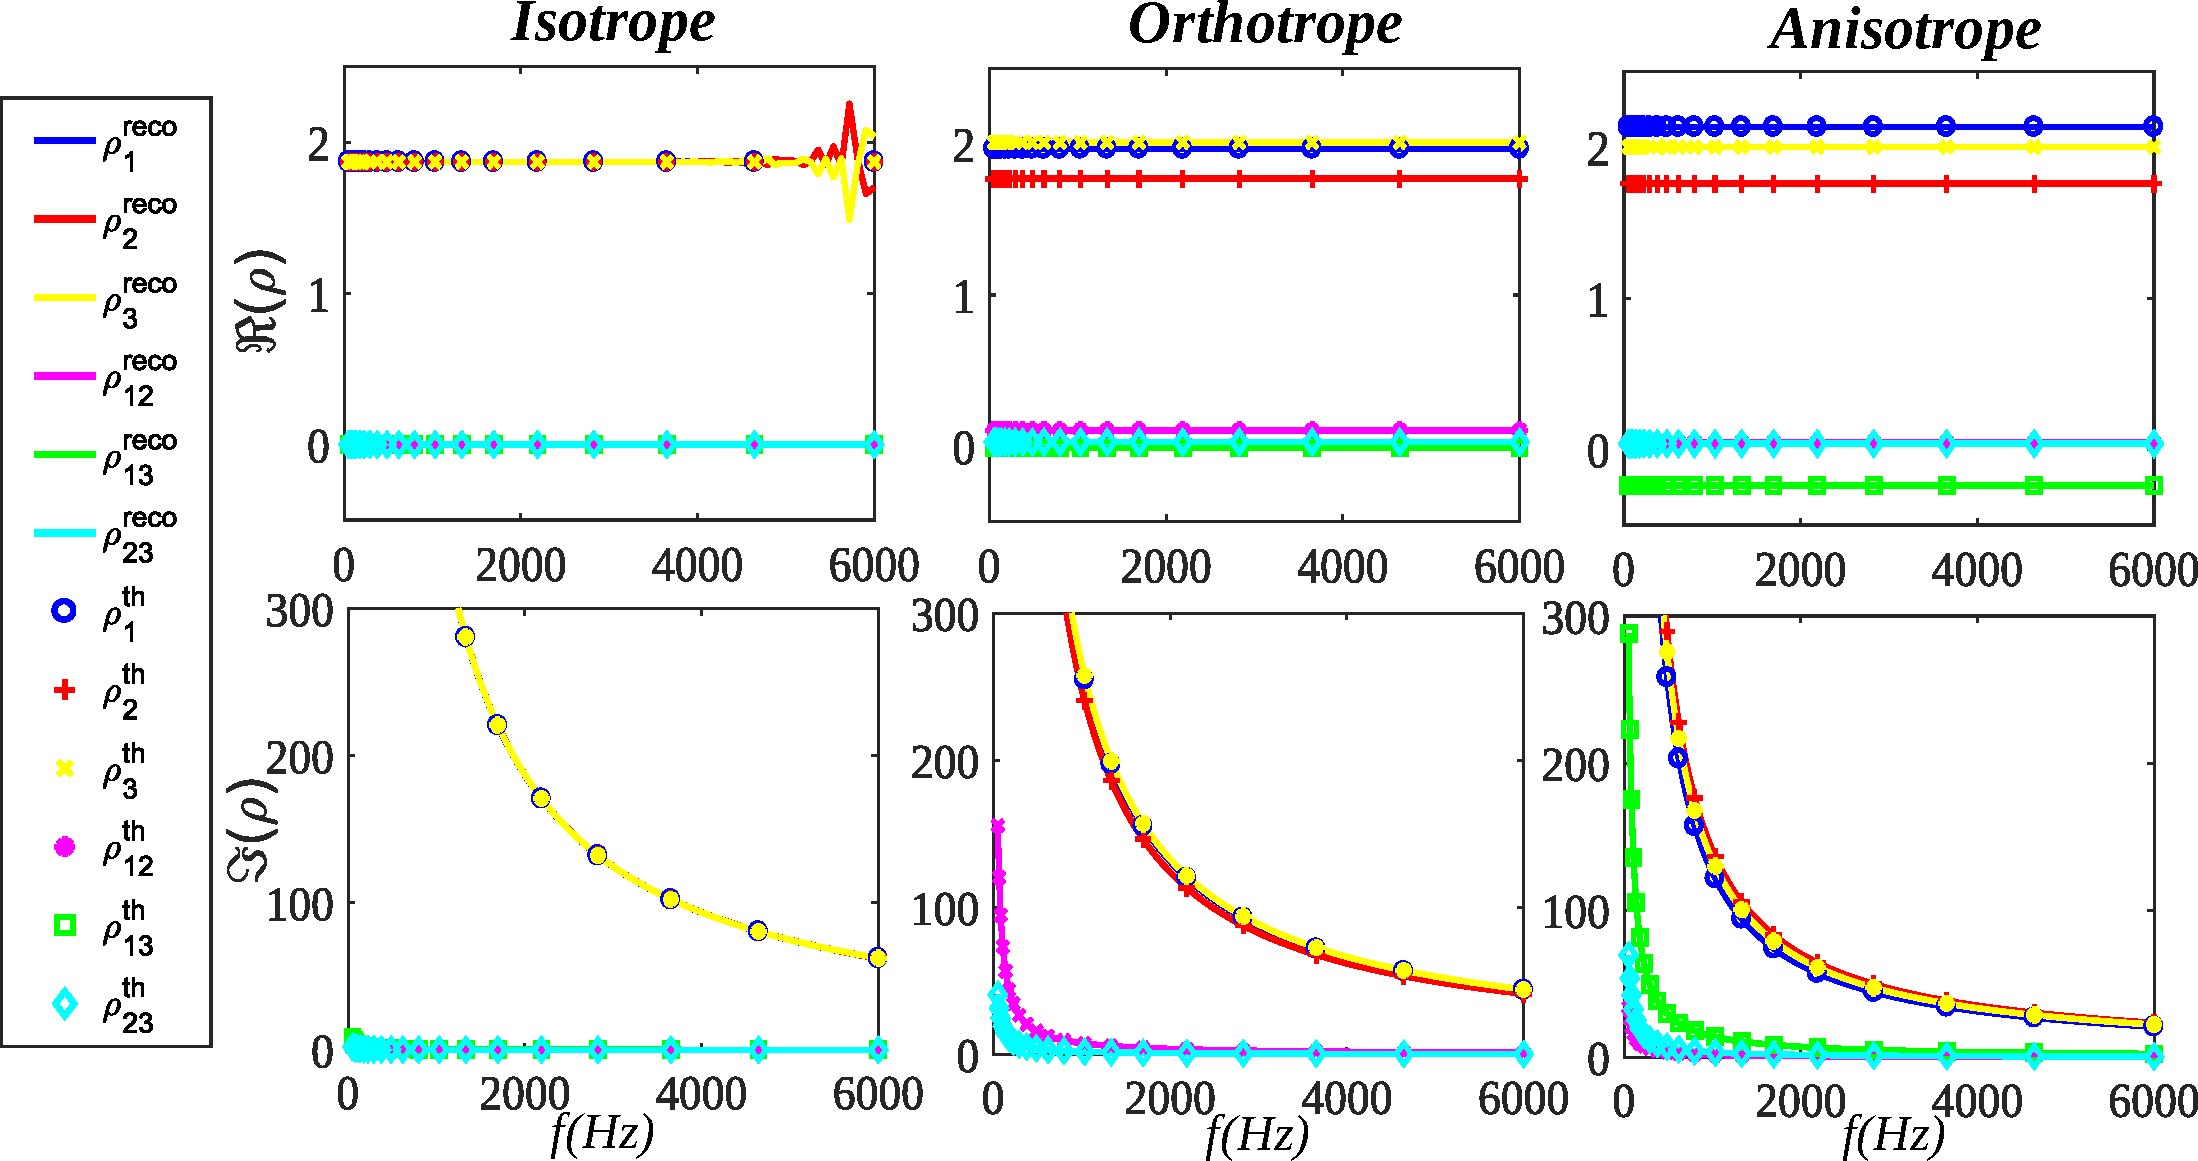
\includegraphics[scale=0.45]{Density_rot.pdf}
        \caption{Densités complexes du fluide équivalent (marqueurs rond) et reconstruites par méthode inverse  (lignes continues), dans le cas isotrope, orthotrope et anistrope, en utilisant  incidence non-nulles. Les coefficients R et T utilisé pour la reconstruction sont ici sans bruit.}
        \label{rho_rot}
    \end{figure}
    
    De même que pour le bulk mudulus, la méthode donne une identification parfaite des densités complexes dans le cas sans bruit, conformément aux au faits d'utiliser le même modèle pour l'obtention de R et T et pour l'obtention de la méthode inverse. Une observation possible sur le matériau poreux anisotrope et orthotrope est que la partie imaginaire des densités diagonales sont très proches, ce qui peut jouer un rôle dans l'identification des directions principales du matériau.
    
    Par une simple diagonalisation de la matrice de densité $\bar{\bar{\rho}}$, il est possible de retrouver les densités dans les directions principales. Et en utilisant des critères de rangement des valeurs propres, il est possible de retrouver, à partir des vecteurs propres triés, les angles de rotations des directions principales. Dans notre cas la fonction "rotm2eul" de $matlab^{\textregistered}$, avec comme critère de tri des valeurs propres $0<\theta_{I}<\frac{\pi}{2}$ et $0<\theta_{II}<\frac{\pi}{2}$.
    Les densités complexes des directions principales et les angles de rotation obtenu dans les trois cas isotrope, orthotrope et anisotrope sont représentés sur la figure (\ref{rho_dir}) : 
    \begin{figure}[ht!]
        \centering
        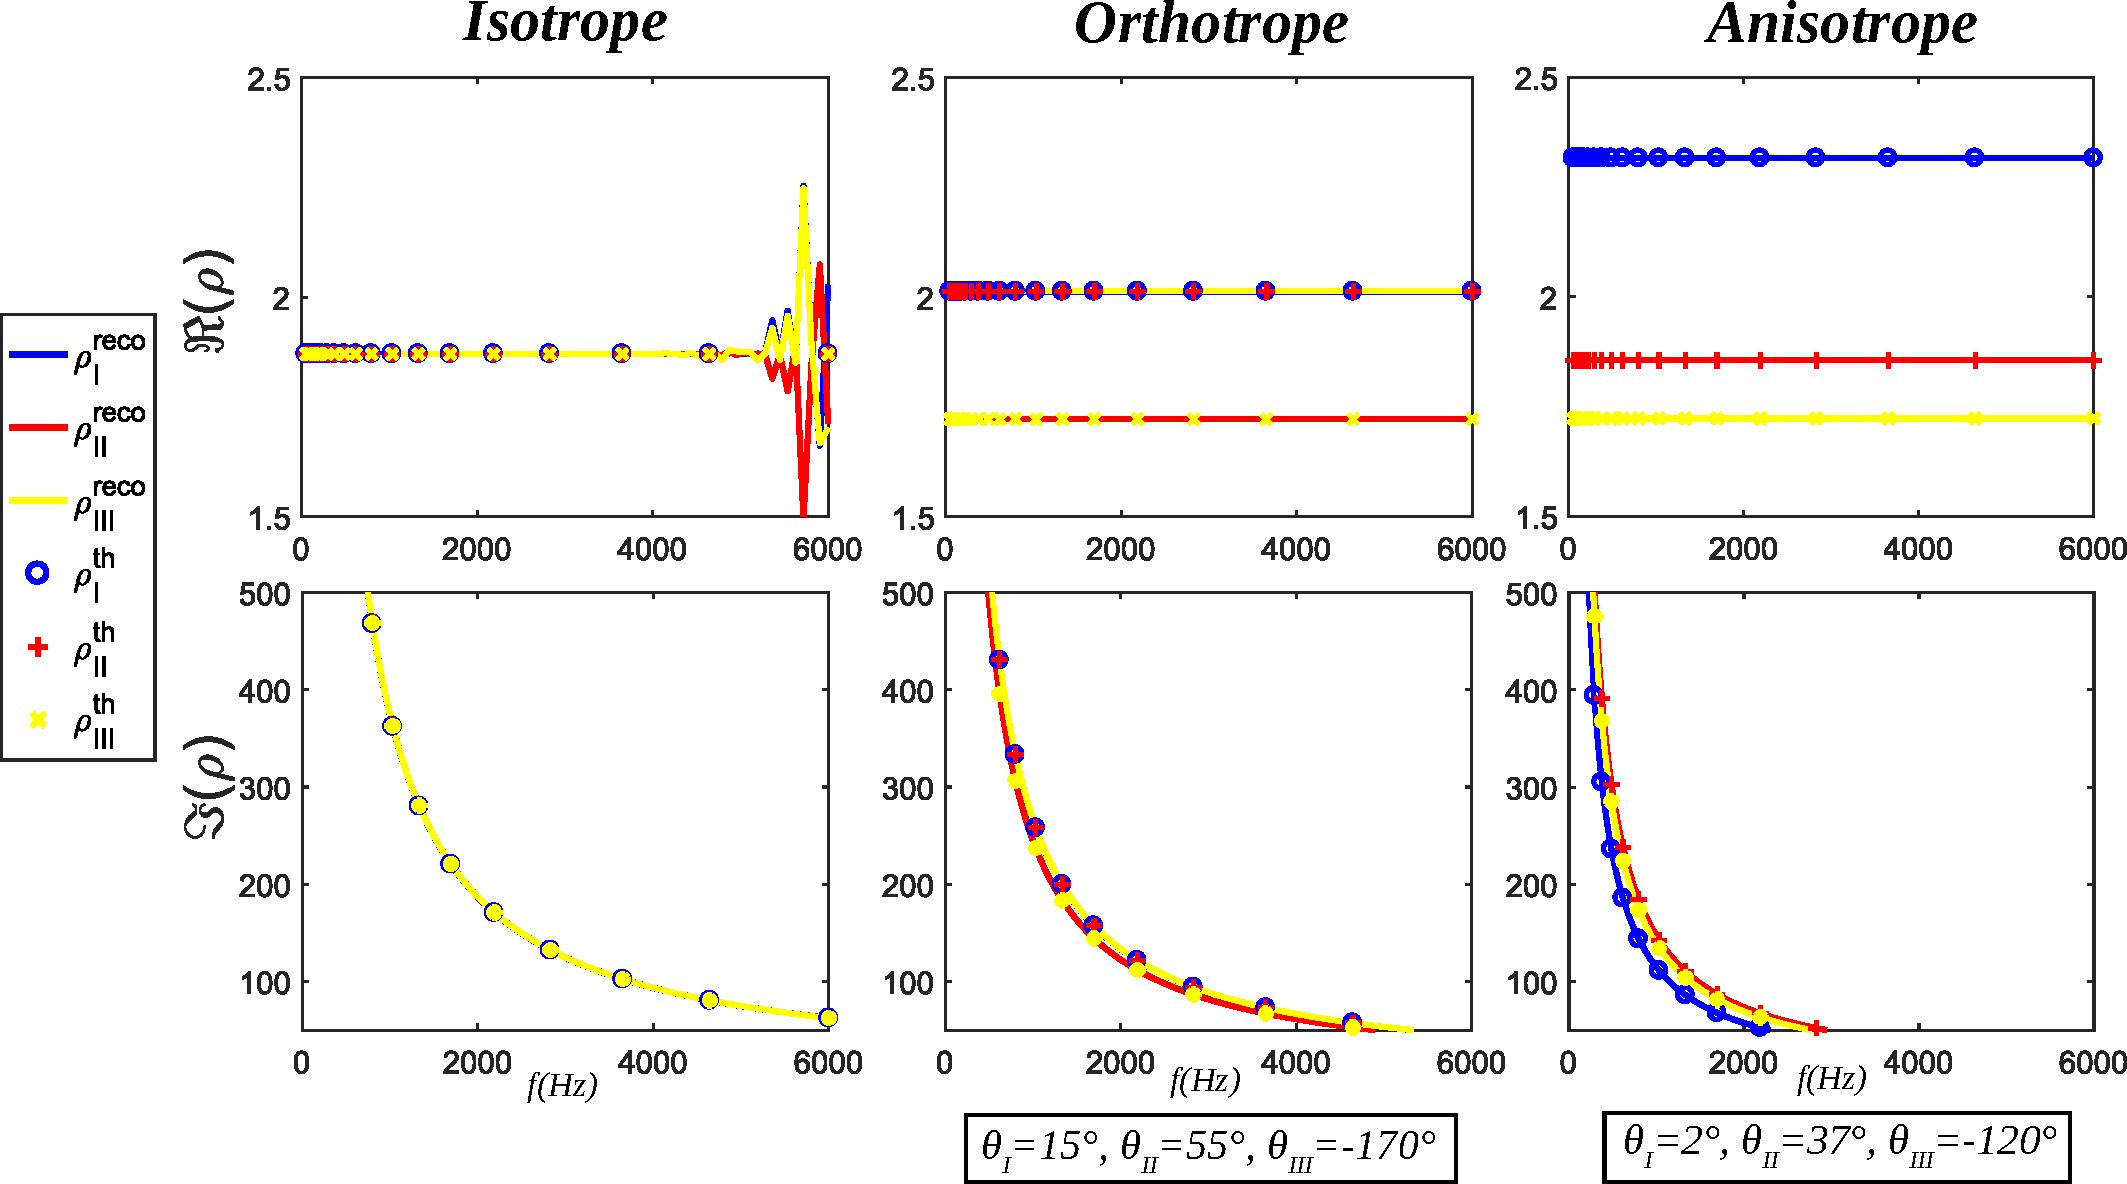
\includegraphics[scale=0.45]{Density_dir.pdf}
        \caption{Densités dan les directions princiaples de la couche fluide équivalent (marqueurs rond) et reconstruites par méthode inverse  (lignes continues), dans le cas isotrope, orthotrope et anistrope. Les coefficients R et T utilisé pour la reconstruction sont ici sans bruit.}
        \label{rho_dir}
    \end{figure}
    
    La reconstruction est identique aux densités du fluide équivalent, a part pour le cas isotrope où l'on retrouve la même irrégularité que précédemment. Dans le cas anisotrope, les densités dans les directions principales sont triées le même ordre que pour le fluide équivalent et l'on retrouve les trois angles d'euler comme introduit dans le milieu étudié. Il est ici rappelé que les densités correspondent a des plans, qui sont donc $\pi$ périodique et l'on retrouve bien : $\theta_{III}=-120°=60°$. Dans le cas du fluide équivalent poreux, les densités $\rho_{II}$ et $\rho_{III}$ sont permuté en comparaison au paramètres initiaux du milieu, cette permutation peut être observé par un déphasage de $\frac{\pi}{2}$ sur l'angle $\theta_{III}$.
    
    Des signaux bruité sont maintenant utilisé pour l'identification des paramètres des paramètres des mêmes trois matériaux poreux isotrope, orthotrope et anisotrope. Le bruit est introduit par l'ajout de valeur décrits en terme de module phase. Le module du bruit dépend d'une loi gaussienne centrée sur la valeur cible et sa phase dépend d'une loi uniforme entre 0 et $3\pi$. La valeur cible ici choisie est l'énergie non-absorbée par le système, c'est-à-dire $|1-\alpha|$, où $\alpha$ est l'absorption du milieu. Le bruit est ainsi ajouté au différents R et T et un exemple de coefficients obtenus est tracé sur la figure (\ref{RT_noise}). 
    
    \begin{figure}[ht!]
        \centering
        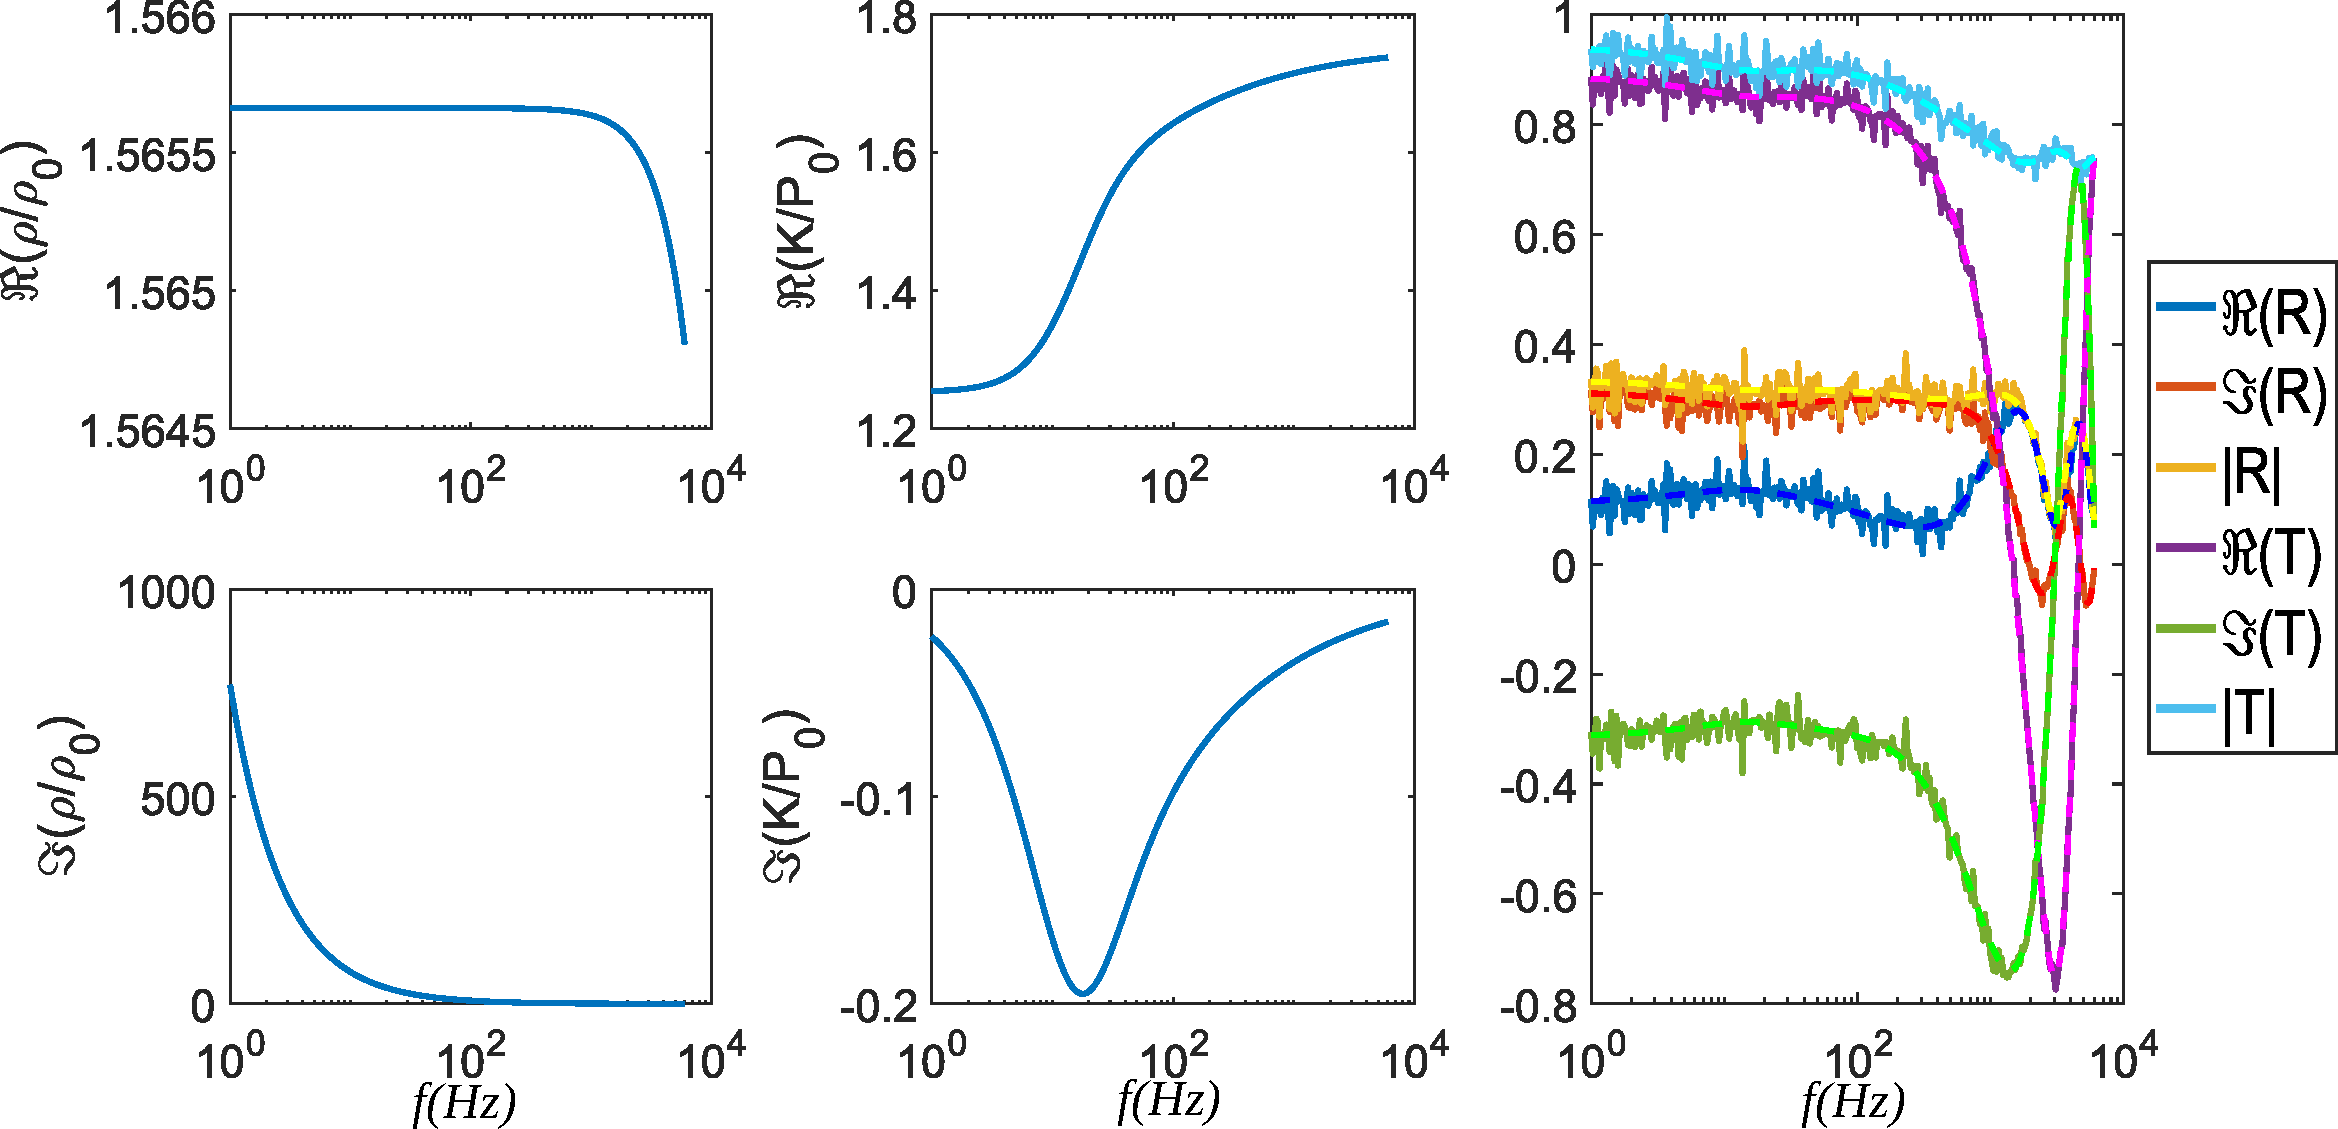
\includegraphics[scale=0.45]{RT_noise.pdf}
        \caption{Coefficient de réflection R et de transmission simulés pour un fluides équivalent anisotropes dont la matrice densité et le bulk sont représenté a gauche de la figure. Les coefficients R et T sont tracé dans le cas sans bruit (marqueurs rond) et avec un bruit introduit (ligne continue) pour un SNR de 30 dB}
        \label{RT_noise}
    \end{figure}
    
    L'identification des paramètres peut être fait pour différents niveaux de bruit, suivant la même méthode que dans le cas sans bruit sans ajouter de régularisation. La méthode est appliquée pour deux cas de matériaux poreux, isotrope et anisotrope, afin d'avoir deux cas représentatif dans les axes principaux (isotrope) et hors des directions principales (anisotropes). Les paramètres reconstruits représentés dans la suite sont le bulk modulus et les densités $\rho_1$, $\rho_{13}$ et $\rho_3$. Ce choix de densités correspond est fait pour simplifier l'analyse de la méthode soumise a du bruit, il permet d'observer l'identification de paramètres en incidence normale ($\rho_3$ et K), en incidence oblique ($\rho_1$ et $\rho_{13}$). 
    
    \begin{figure}[ht!]
        \centering
        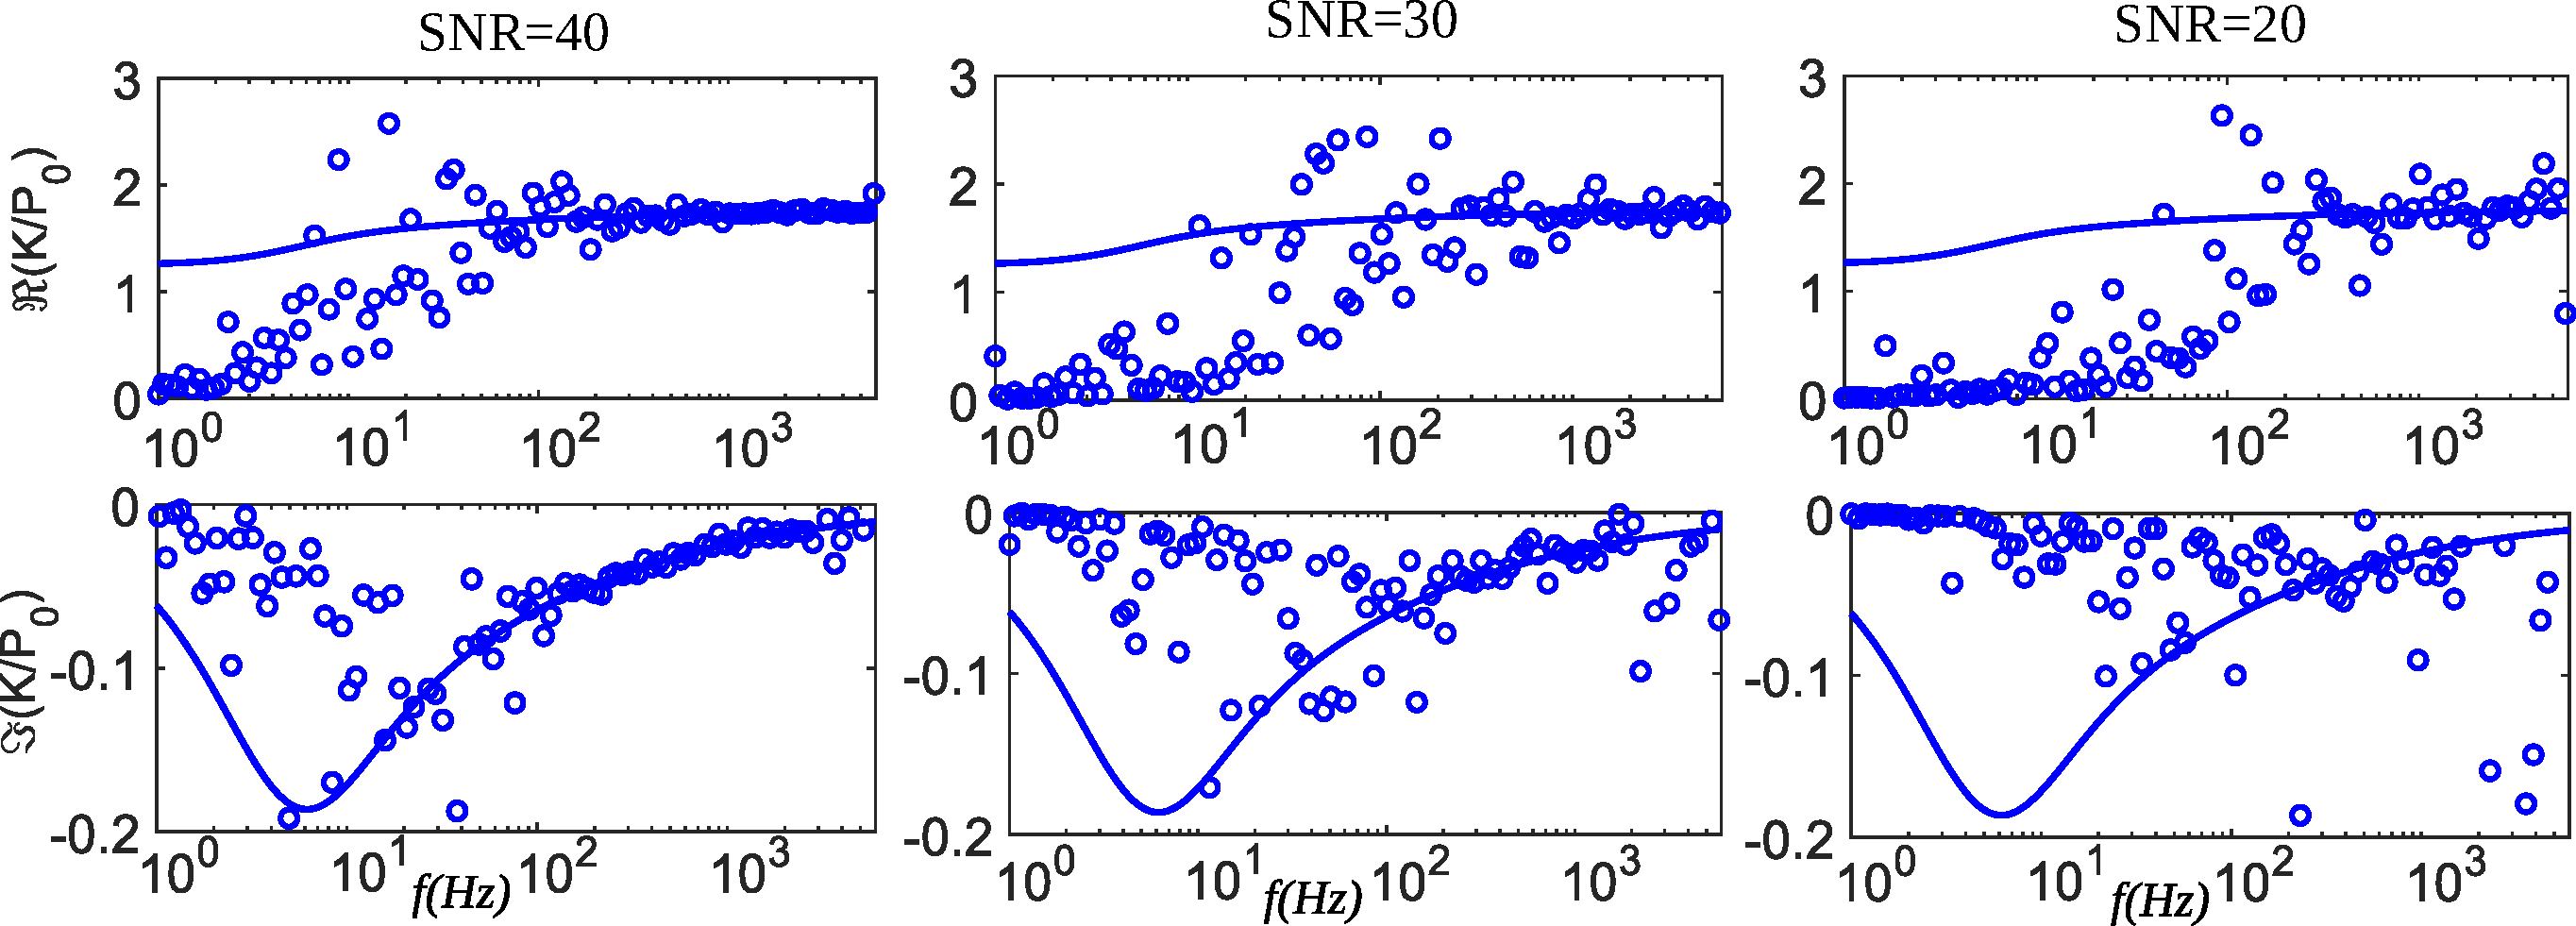
\includegraphics[scale=0.38]{Bulk_noise.pdf}
        \caption{Identification du bulk modulus pour un fluide équivalent anisotrope à partir de coefficients R et T soumis a trois niveaux de bruit différents. Les bulk modulus identifiés (marqueurs ronds) sont comparés aux bulk modulus du fluide équivalent (ligne continue). La reconstruction dans les trois cas est pertinente à partir de 100 Hz, après la phase de transition du bulk modulus.}
        \label{bulk_noise}
    \end{figure}
    
    Le premier paramètre reconstruit est le bulk modulus, l'identification est faites dans le cas du fluide équivalent anisotrope, pour trois SNR(rapport signal sur bruit) de 20, 30 et 40 dB. Les différents bulk obtenus sont représenté sur la figure (\ref{bulk_noise}). Logiquement avec l'augmentation du niveau de bruit, l'identification devient moins performante, mais il est possible de voir deux domaines dans la reconstruction du bulk modulus. Le premiers la transition du bulk modulus à 100 Hz, où la reconstruction est relativement fidèle et le second avant la transition où même avec un faible niveau de bruit la reconstruction est fausse.
    
    Les densités sont ensuite reconstruites dans le cas isotrope, pour les mêmes R et T.   
\begin{figure}[ht!]
        \centering
        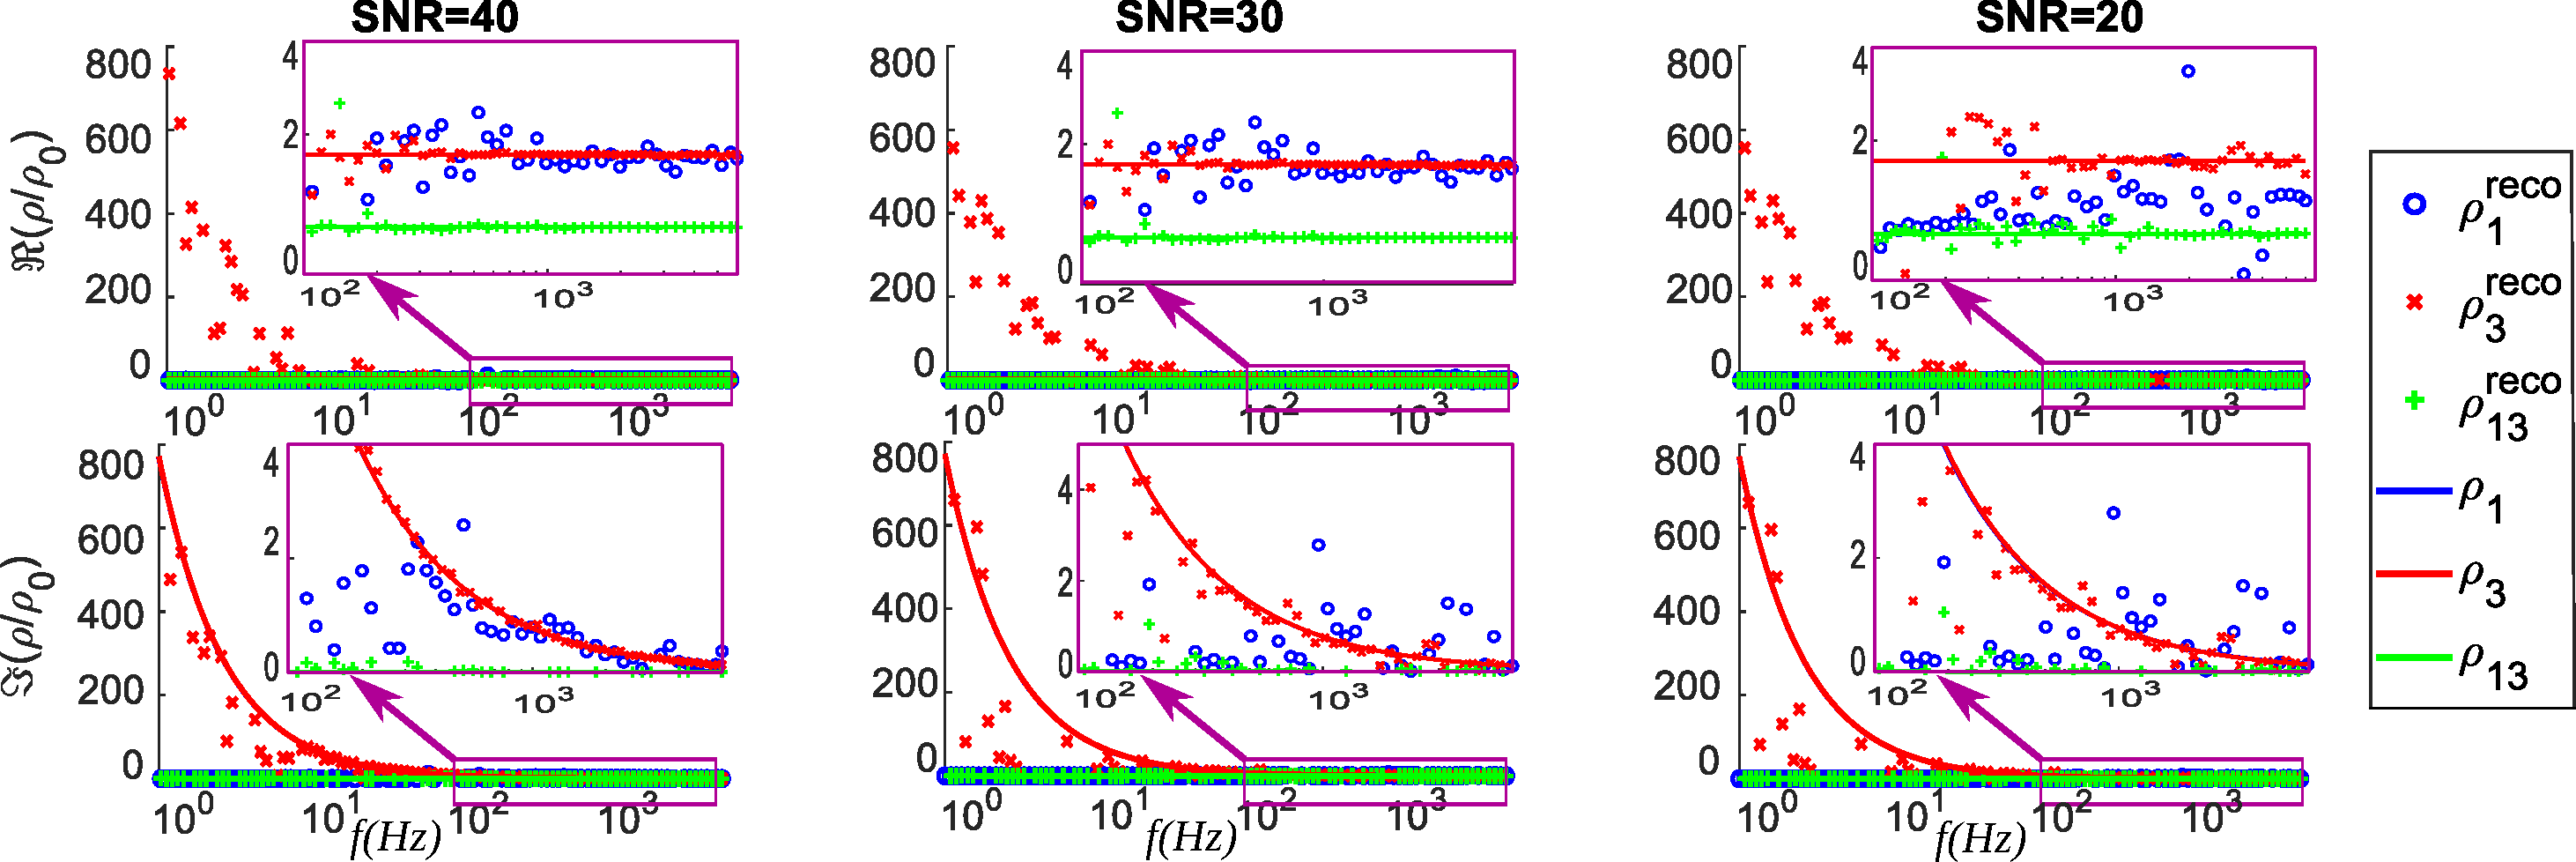
\includegraphics[scale=0.38]{Density_iso_noise.pdf}
        \caption{Caption}
        \label{fig:my_label}
    \end{figure}
\begin{figure}[ht!]
        \centering
        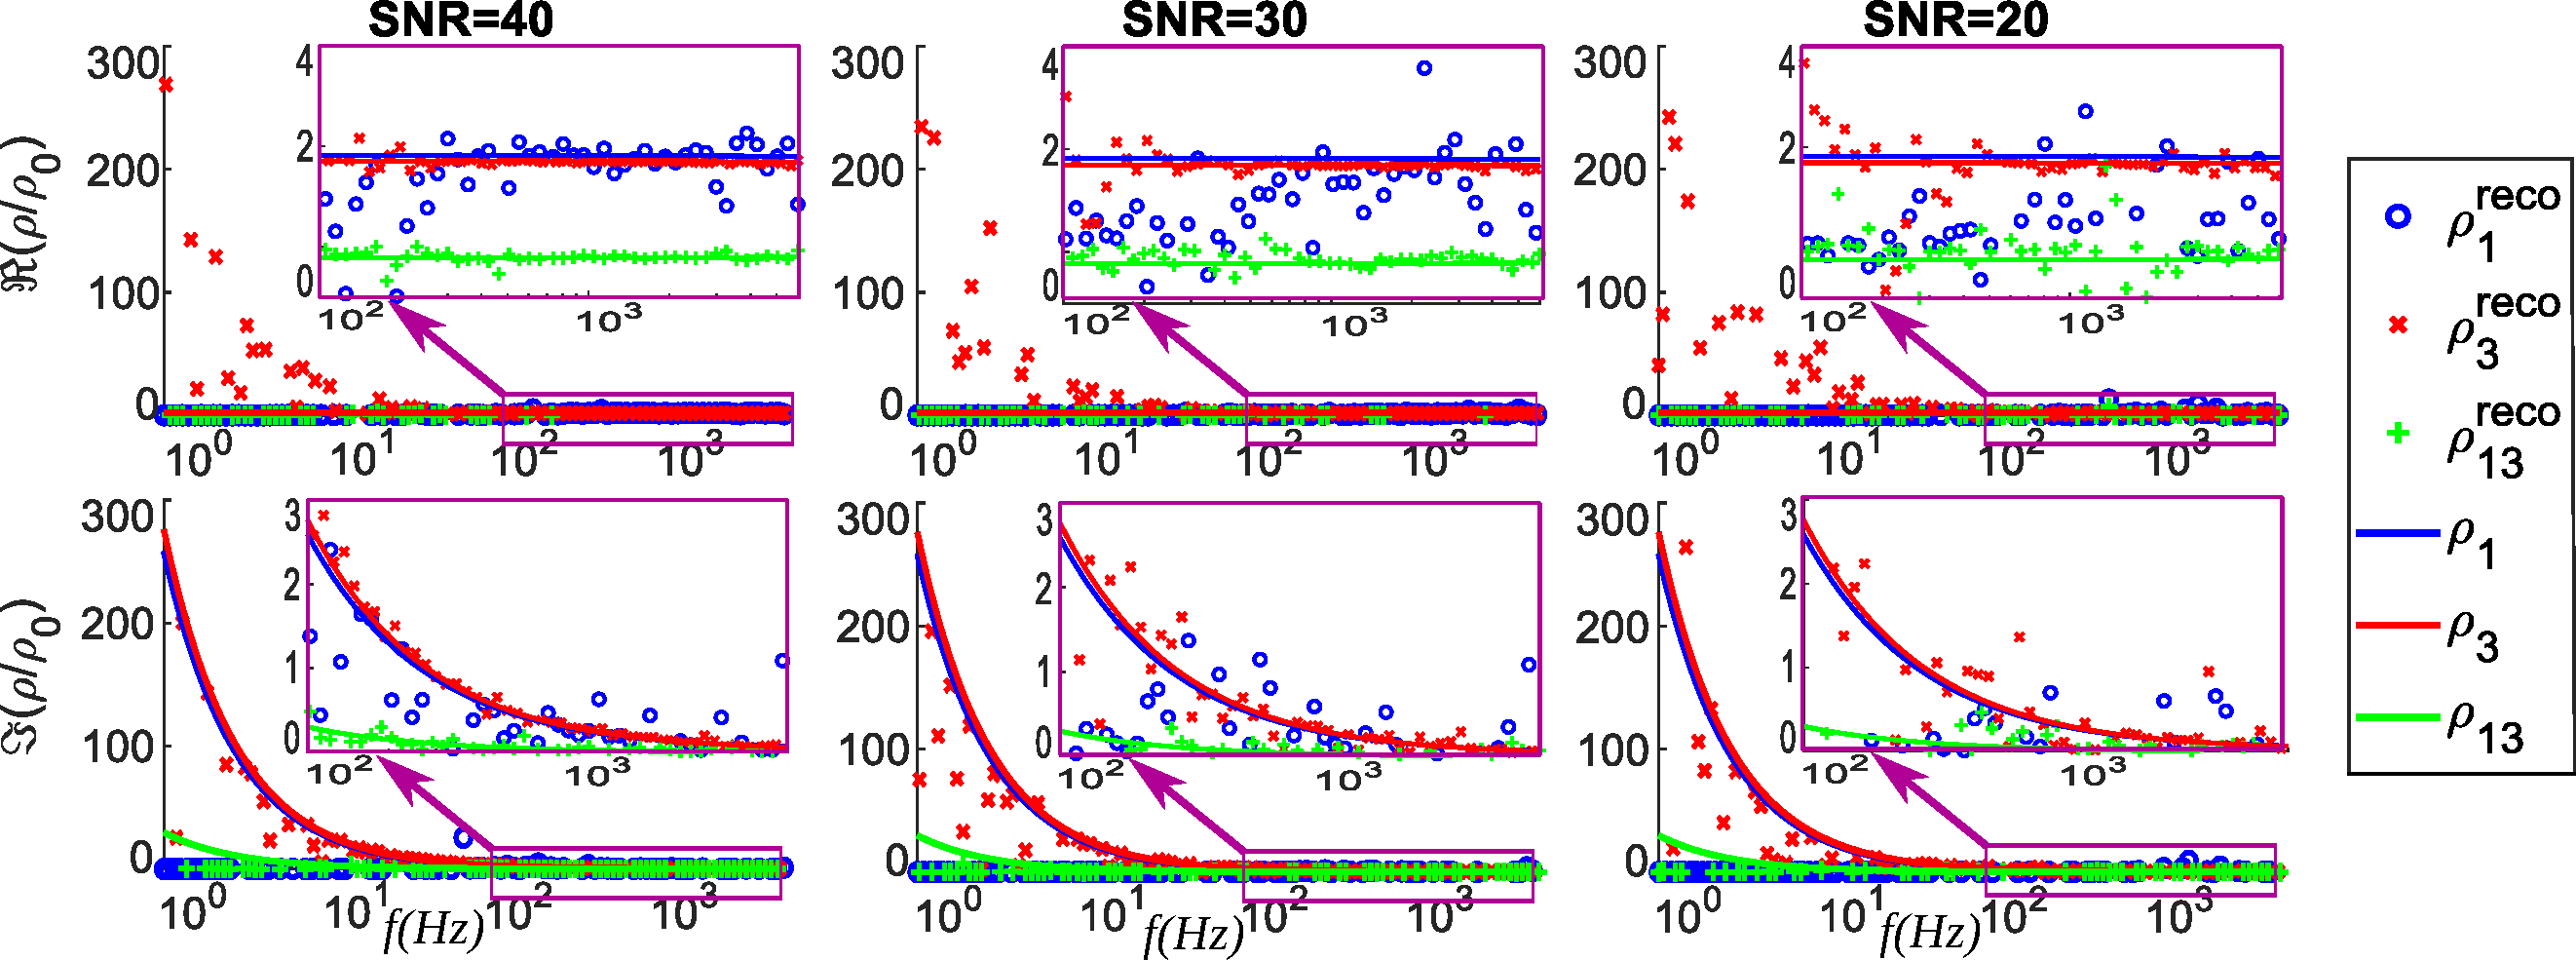
\includegraphics[scale=0.38]{Density_anis_noisy.pdf}
        \caption{Caption} 
        \label{fig:my_label}
    \end{figure}

%%%%%%%%%%%%%%%%%%%%%%%%%%%%%%%%%%%%%%%%%%%%%%%%%%%%%%%%%%%%%%%%%%%%%%%%%%%%%%%%%%%%%%%%%%%%%%%%%%%%%%%%%%%%%%%%%%%%%%%%%%%%%%%%%%%%%%%%%%%%
\chapter*{Conclusion}
\addcontentsline{toc}{chapter}{Conclusion}  


%%%%%%%%%%%%%%%%%%%%%%%%%%%%%%%%%%%%%%%%%%%%%%%%%%%%%%%%%%%%%%%%%%%%%%%%%%%%%%%%%%%%%%%%%%%%%%%%%%%%%%%%%%%%%%%%%%%%%%%%%%%%%%%%%%%%%%%%%%%%
\bibliography{Biblio.bib}
\addcontentsline{toc}{chapter}{Bibliographie} 

%%%%%%%%%%%%%%%%%%%%%%%%%%%%%%%%%%%%%%%%%%%%%%%%%%%%%%%%%%%%%%%%%%%%%%%%%%%%%%%%%%%%%%%%%%%%%%%%%%%%%%%%%%%%%%%%%%%%%%%%%%%%%%%%%%%%%%%%%%%%
\chapter*{Annexes}
\addcontentsline{toc}{chapter}{Annexe} 
\section*{Annexe A : Rotation des directions principales du milieu fluide équivalent}
\label{Ch_Ann_S_rot}

    La rotation du milieu fluide équivalent anisotrope est faites selon les 3 angles d'Euler $\theta_{III}$, $\theta_{II}$ et $\theta_{I}$, représentés sur la figure (\ref{Porous_Mat}), autour des axes $x_3$, $x_2$ et $x_1$. Les trois matrices de rotation associées sont :
    \begin{align}
        &R_{III}=R(\theta_{III})=\begin{pmatrix} 
                                    cos(\theta_{III}) & -sin(\theta_{III}) & 0 \\
                                    sin(\theta_{III}) & cos(\theta_{III}) & 0 \\
                                    0 & 0 & 1
                                \end{pmatrix},\\
        &R_{II}=R(\theta_{II})=\begin{pmatrix} 
                                    cos(\theta_{II}) & 0 & +sin(\theta_{II})\\
                                    0 & 1 & 0 \\
                                    -sin(\theta_{II}) & 0 & cos(\theta_{II})
                                \end{pmatrix},\\
        &R_{I}=R(\theta_{I})=\begin{pmatrix} 
                                    1 & 0 & 0\\
                                    0 & cos(\theta_{I}) & -sin(\theta_{I}) \\
                                    0 & sin(\theta_{I}) & cos(\theta_{I}) 
                                \end{pmatrix}.\\
    \end{align}
    
    Considérant  les propriétés des matrices de rotation, il est possible d'écrire la matrice de rotation global comme :
    
\hspace{-3cm}
\begin{changemargin}{-2.8cm}{-1cm}
    \begin{align}
    R &=R_{III}*R_{II}*R_{I}\\
      &=\begin{pmatrix}
        cos(\theta_{II})cos(\theta_{III}) & -sin(\theta_{III})cos(\theta_{I})-sin(\theta_{I})sin(\theta_{II})cos(\theta_{III}) & sin(\theta_{I})sin(\theta_{III})-sin(\theta_{II})cos(\theta_{I})cos(\theta_{III})\\
        sin(\theta_{III})cos(\theta_{II}) & cos(\theta_{I})cos(\theta_{III})-sin(\theta_{I})sin(\theta_{II})sin(\theta_{III}) & -sin(\theta_{I})cos(\theta_{III})-sin(\theta_{II})sin(\theta_{III})cos(\theta_{I}) \\
        sin(\theta_{II}) & sin(\theta_{I})cos(\theta_{II}) & cos(\theta_{I})cos(\theta_{II})
                                \end{pmatrix}.\nonumber
    \end{align}
\end{changemargin}

    La  matrice rotation peut s'appliquer à la matrice de densité complexe, qui devient :
    \begin{align}
        \bar{\bar{\rho_{rot}}}=R\bar{\bar{\rho}}R^{-1}.
    \end{align}
    
    
\end{document}